\documentclass[a4paper]{article}
\usepackage{geometry}
\geometry{left=1.8cm,right=1.8cm,top=1.8cm,bottom=1.8cm}
\usepackage{ctex}
\usepackage{graphicx,subcaption}
\usepackage{amssymb}
\usepackage{indentfirst}
\usepackage{amsmath}
\usepackage{amsthm}
\usepackage{bm}
\usepackage{lineno}
\usepackage{setspace}
\usepackage{booktabs,multirow}
\usepackage{authblk}
\usepackage{float}
\usepackage{placeins}
\setlength{\textfloatsep}{8pt plus 1pt minus 2pt}
\setlength{\floatsep}{8pt plus 1pt minus 2pt}
\setlength{\intextsep}{8pt plus 1pt minus 2pt}
\usepackage[flushleft]{threeparttable}
\usepackage{listings}
\usepackage{xcolor}
\usepackage{enumitem}
\usepackage{array}

\lstset{
    language=C++,
    basicstyle=\ttfamily\small,
    keywordstyle=\color{blue}\bfseries,
    stringstyle=\color{red},
    commentstyle=\color{green!50!black}\itshape,
    numberstyle=\tiny,
    stepnumber=1,
    numbersep=5pt,
    showspaces=false,
    showstringspaces=false,
    frame=single,
    breaklines=true,
    tabsize=4
}

\usepackage[colorlinks,citecolor=blue,urlcolor=blue]{hyperref}

\newtheorem{theorem}{Theorem}
\newtheorem{lemma}[theorem]{Lemma}

\newcommand{\E}{\mathrm{E}}
\newcommand{\Var}{\mathrm{Var}}
\newcommand{\Cov}{\mathrm{Cov}}
\newcommand{\tr}{\mathrm{tr}}
\newcommand{\iid}{\mathrm{i.i.d.}\ }
\newcommand{\normtwo}[1]{\|#1\|_2}
\newcommand{\norminf}[1]{\|#1\|_\infty}
\newcommand{\eps}{\varepsilon}
\newcommand{\upk}[1]{^{(#1)}}

\title{\textbf{3DGS 物理效果模拟实验报告}}
\author{李亭皑\quad PB23010374}
\date{\today}

\doublespacing

\begin{document}

\maketitle

\begin{abstract}
本文围绕 3D Gaussian Splatting 场景的物理效果模拟，分别实现并比较显式 MPM、隐式 MPM 和 PBMPM 三类求解器。实验在统一花盆场景下考察网格分辨率、时间步长、隐式容差以及 PBMPM 参数对稳定性、计算代价和运动质量的影响，并结合渲染关键帧分析不同方法的典型失效和调参规律。
\end{abstract}

\section{问题背景}

\subsection{3DGS 重建原理}

三维高斯泼溅是一种显式的三维场景表示方法。它通常从多视角图像和稀疏点云出发，将每个空间点初始化为一个三维高斯核，并为每个高斯核维护位置、协方差、不透明度和视角相关颜色等参数。训练时，方法通过可微渲染将这些三维高斯投影到图像平面，并将渲染结果与真实图像比较，从而反向优化高斯的位置、形状、透明度和颜色 \cite{kerbl2023gaussian}。

3DGS 中的颜色由球谐函数表示的视角相关函数。对第 $p$ 个 Gaussian，记从 Gaussian 中心指向相机的单位观察方向为 $\bm{d}\in\mathbb{S}^2$，则其颜色可以写成
\[
    \bm{c}_p(\bm{d})
    =
    \sum_{\ell=0}^{L}
    \sum_{m=-\ell}^{\ell}
    \bm{c}_{p,\ell m}
    Y_{\ell m}(\bm{d}),
\]
其中 $Y_{\ell m}$ 是定义在单位球面上的球谐基函数，$\bm{c}_{p,\ell m}\in\mathbb{R}^3$ 是对应的 RGB 系数。$0$ 阶项表示与视角无关的基础颜色，高阶项刻画随观察方向变化的外观。因此，3DGS 可以在不显式建立光照、法线和材质模型的情况下，用每个 Gaussian 携带的球谐系数近似视角相关颜色。

3DGS 选择高斯核作为基本图元，与高斯分布本身的封闭性质有关。设一个三维高斯核的中心为 $\bm{\mu}$，协方差矩阵为 $\bm{\Sigma}$。在仿射变换
\[
    \bm{x}'=\bm{A}\bm{x}+\bm{b}
\]
下，它仍然是高斯核，其中心和协方差分别变为
\[
    \bm{\mu}'=\bm{A}\bm{\mu}+\bm{b}, \qquad
    \bm{\Sigma}'=\bm{A}\bm{\Sigma}\bm{A}^{T}.
\]
因此，各向异性高斯椭球经过旋转、缩放和平移后，仍然可以用新的中心和协方差矩阵表示。这一点使得 3DGS 可以用协方差矩阵描述局部椭球形状，并在物体运动或局部仿射形变后继续保持高斯图元的形式。

高斯核在边缘化和积分下也具有封闭性。对三维高斯沿一个坐标方向积分，可以得到二维高斯。因此，当一个三维高斯椭球被投影到图像平面时，它在屏幕上的影响区域可以近似表示为一个二维椭圆高斯。需要注意的是，真实透视投影并不是严格的仿射变换，所以 3DGS 采用局部线性化的方式：在每个高斯中心附近，用投影函数的雅可比矩阵近似透视投影，再计算屏幕空间的二维协方差。若相机变换矩阵为 $\bm{W}$，投影局部雅可比矩阵为 $\bm{J}$，则投影后的协方差可写成
\[
    \bm{\Sigma}'=\bm{J}\bm{W}\bm{\Sigma}\bm{W}^{T}\bm{J}^{T}.
\]
随后取其图像平面上的 $2\times 2$ 部分作为二维高斯泼溅图元的协方差。

\section{开源项目仿真原理}

\subsection{PhysGaussian :显式 MPM 更新}

PhysGaussian 将重建得到的三维高斯核直接视为连续体的离散材料点，因此同一批 Gaussian 既参与物理仿真，也参与后续渲染，避免了从渲染几何到仿真网格的额外嵌入过程 \cite{xie2024physgaussian}。对第 $p$ 个材料点，记其位置、速度、质量、体积、形变梯度、仿射速度矩阵分别为 $\bm{x}_p^n$、$\bm{v}_p^n$、$m_p$、$V_p^0$、$\bm{F}_p^n$ 和 $\bm{C}_p^n$；对第 $i$ 个网格节点，记其位置、质量和速度为 $\bm{x}_i$、$m_i^n$ 和 $\bm{v}_i^n$。粒子与网格之间通过 $B$ 样条插值权重传递信息，记
\[
    w_{ip}^n = N\left(\frac{\bm{x}_i-\bm{x}_p^n}{\Delta x}\right),
\]
其中 $N$ 是紧支撑 $B$ 样条核函数，$\Delta x$ 是网格间距。一次显式 MPM 子步可以概括为 $P2G$、网格更新和 $G2P$ 三个阶段。

在 $P2G$ 阶段，粒子质量和动量被加权转移到附近网格节点。PhysGaussian 采用 APIC 形式的动量传递，即
\[
    m_i^n = \sum_p w_{ip}^n m_p,
\]
\[
    m_i^n \bm{v}_i^n
    =
    \sum_p w_{ip}^n m_p
    \left(
        \bm{v}_p^n
        +
        \bm{C}_p^n(\bm{x}_i-\bm{x}_p^n)
    \right).
\]
其中 $\bm{C}_p^n(\bm{x}_i-\bm{x}_p^n)$ 描述粒子局部仿射速度场对网格节点的贡献，相比只传递平移动量的 PIC 方法，它能更好地保留局部旋转和剪切信息。

随后在网格上进行显式速度更新。设 $\bm{\tau}_p^n$ 为由材料模型和形变梯度计算得到的 Kirchhoff 应力，外力为 $\bm{f}_i^{\mathrm{ext},n}$，则内力可写为
\[
    \bm{f}_i^{\mathrm{int},n}
    =
    -
    \sum_p V_p^0 \bm{\tau}_p^n \nabla w_{ip}^n.
\]
显式 Euler 更新为
\[
    \bm{v}_i^{n+1}
    =
    \bm{v}_i^n
    +
    \Delta t\,
    \frac{
        \bm{f}_i^{\mathrm{int},n}
        +
        \bm{f}_i^{\mathrm{ext},n}
    }{m_i^n}.
\]

在 $G2P$ 阶段，更新后的网格速度被插值回粒子，并推进粒子状态：
\[
    \bm{v}_p^{n+1}
    =
    \sum_i w_{ip}^n \bm{v}_i^{n+1},
\]
\[
    \bm{x}_p^{n+1}
    =
    \bm{x}_p^n + \Delta t\,\bm{v}_p^{n+1}.
\]
同时由网格速度梯度更新形变梯度：
\[
    \nabla \bm{v}_p^{n+1}
    =
    \sum_i \bm{v}_i^{n+1}(\nabla w_{ip}^n)^{T},
\]
\[
    \bm{F}_p^{n+1}
    =
    \left(\bm{I}+\Delta t\,\nabla \bm{v}_p^{n+1}\right)\bm{F}_p^n.
\]
若材料包含塑性，还需要对试探形变梯度施加 return mapping，将其投影回材料允许的弹性区域：
\[
    \bm{F}_p^{n+1}
    \leftarrow
    \mathcal{Z}\left(\bm{F}_p^{n+1}\right).
\]

\subsection{仿真结果到高斯核的作用方式}

物理仿真得到的是每个材料点的平移和局部一阶形变。对于三维高斯核而言，设静态重建时第 $p$ 个 Gaussian 在材料空间中的中心和协方差为 $\bm{X}_p$ 与 $\bm{A}_p$。若局部形变可由一阶近似表示为
\[
    \bm{x}
    \approx
    \bm{x}_p(t)
    +
    \bm{F}_p(t)(\bm{X}-\bm{X}_p),
\]
则由高斯核的仿射不变性可知，变形后的 Gaussian 仍然是 Gaussian，并且其中心与协方差更新为
\[
    \bm{x}_p(t)=\phi(\bm{X}_p,t),
    \qquad
    \bm{A}_p(t)
    =
    \bm{F}_p(t)\bm{A}_p\bm{F}_p(t)^{T}.
\]
这正是 PhysGaussian 可以将 MPM 的一阶运动直接作用到 3DGS 核上的原因：MPM 提供每个材料点的中心运动和局部形变梯度，而高斯核在局部仿射变换下仍保持可渲染的高斯形式。实际实现中，也可以采用增量形式更新协方差：
\[
    \bm{A}_p^{n+1}
    =
    \bm{A}_p^n
    +
    \Delta t
    \left(
        \nabla \bm{v}_p^n \bm{A}_p^n
        +
        \bm{A}_p^n(\nabla \bm{v}_p^n)^{T}
    \right),
\]
该形式不需要显式保存从初始状态到当前状态的总形变梯度。

对于颜色，3DGS 的颜色通常是视角相关的，若物体发生旋转而球谐方向仍固定在世界坐标系中，则同一材料表面在相对观察方向不变时也可能出现不合理的颜色变化。因此，PhysGaussian 从形变梯度的极分解
\[
    \bm{F}_p = \bm{R}_p\bm{S}_p
\]
中提取局部旋转 $\bm{R}_p$，并用反向旋转后的观察方向计算球谐颜色：
\[
    f_p^t(\bm{d})
    =
    f_p^0(\bm{R}_p^{T}\bm{d}).
\]
这样做等价于让球谐基函数的方向随物体局部旋转，而球谐系数本身仍然附着在材料点上。对于近似漫反射颜色，这一旋转影响较小；对于高阶球谐表示的视角相关外观，它可以使高光和方向性颜色变化与物体运动保持一致。最终，每一帧只需用更新后的 $\bm{x}_p(t)$、$\bm{A}_p(t)$、$\alpha_p$ 和旋转后的球谐颜色进入原始 3DGS 渲染管线，即可得到物理驱动的新视角动态渲染结果。

\section{本项目概述}

本项目基于开源 3DGS Web 渲染引擎 SuperSplat 搭建交互式前端，在原有静态 Gaussian 查看、选择和编辑功能之上增加物理仿真入口，并使用 PhysGaussian 作为 baseline 仿真后端。前端负责模型加载、区域选择、材料参数设置、边界条件设置和求解器选择，并将用户交互转换为统一的物理仿真配置
\[
    \Theta
    =
    \left(
        E,\nu,\rho,\Delta t,h,\mathcal{B},\mathcal{C}
    \right),
\]
其中 $E$ 为杨氏模量，$\nu$ 为泊松比，$\rho$ 为密度，$\Delta t$ 为仿真步长，$h$ 为网格尺度，$\mathcal{B}$ 表示边界约束，$\mathcal{C}$ 表示外力、碰撞和固定区域等条件。后端根据求解器类型
\[
    k\in
    \left\{
        \texttt{explicit},
        \texttt{implicit},
        \texttt{pbmpm}
    \right\}
\]
调用不同积分器，得到离散时间序列
\[
    \mathcal{T}_k:
    \left(
        \mathcal{G}_0,\Theta
    \right)
    \longmapsto
    \left\{
        \mathcal{G}_t
    \right\}_{t=0}^{T}.
\]
为了提高前端动画播放流畅度，本项目将每一帧中发生运动的 Gaussian 索引及其动态属性写成二进制 motion package。每帧主要记录
\[
    \left(
        \bm{\mu}_p^t,
        \bm{q}_p^t,
        \bm{s}_p^t
    \right),
    \qquad p\in \mathcal{I},
\]
其中 $\mathcal{I}$ 是参与仿真的 Gaussian 索引集合，$\bm{q}_p^t$ 和 $\bm{s}_p^t$ 分别表示由协方差分解得到的旋转和尺度。播放时，前端保持原始颜色、不透明度和其他静态属性常驻显存，只更新位置、旋转和尺度，从而减少数据解析、资源重建和主线程阻塞。

在求解方法上，本项目首先保留 PhysGaussian 的显式 MPM 作为 baseline。其次，参考 i-PhysGaussian 的暂未开源的论文，实现隐式 MPM 版本。此外，本项目根据 Local-Global 思想和 PBMPM 的位置约束式物理过程实现了第三类求解器 PBMPM。

最终实验部分围绕显式 MPM、隐式 MPM 和 PBMPM 三类方法进行对比，并进一步对隐式 MPM 的收敛阈值，以及 PBMPM 中从物理量到投影参数的缩放系数进行实验。

除上述主要模块外，本项目还完善了前端交互编辑功能。对于用户选中的 Gaussian 集合，按住 \texttt{Shift} 时，将当前框选集合 $\mathcal{S}_{\mathrm{new}}$ 与已有选择集合 $\mathcal{S}$ 做并集更新，按住 \texttt{Ctrl} 时，则执行差集更新，此外，项目实现了抓手拖动工具：系统将被拖动的模型区域转换为代理粒子组 $\mathcal{P}_{\mathrm{proxy}}$，并在该代理组上执行显式 MPM 求解。


\section{隐式 MPM 求解器实现}

\subsection{设计动机}

显式 MPM 的核心形式可以抽象为常微分方程
\[
    \dot{\bm{y}}=\bm{f}(\bm{y})
\]
上的显式时间推进：
\[
    \bm{y}^{n+1}
    =
    \bm{y}^{n}
    +
    \Delta t\,\bm{f}(\bm{y}^{n}).
\]
对于线性测试方程 $\dot{y}=\lambda y$，显式 Euler 的放大因子为 $1+\Delta t\lambda$。当 $\lambda<0$ 时，稳定性要求
\[
    |1+\Delta t\lambda|\leq 1,
\]
因此时间步长 $\Delta t$ 受到系统最大刚度特征值的限制。对于高杨氏模量材料、强碰撞或准静态过程，系统会变得刚性，显式方法的稳定域较小，较大的 $\Delta t$ 容易导致速度爆炸、形变梯度奇异或粒子越界。隐式方法将末状态也纳入力平衡条件:
\[
    \bm{y}^{n+1}
    =
    \bm{y}^{n}
    +
    \Delta t\,\bm{f}(\bm{y}^{n+1}),
\]
其稳定性通常更好，但每一步都需要求解非线性方程，因此计算代价明显高于显式方法。故i-PhysGaussian 引入 Newton--GMRES 等数值策略降低求解代价 \cite{cao2026iphysgaussian}。

由于 i-PhysGaussian 论文没有开源，本项目的隐式法实现是在 PhysGaussian 的显式 MPM 框架上，根据论文描述重新构造残差、线性化求解和失败保护策略。

\subsection{隐式残差构造}

本项目在网格自由度上求解隐式位移增量。记第 $i$ 个活跃网格节点的位移增量为
\[
    \Delta \bm{u}_i
    =
    \bm{u}_i^{n+1}-\bm{u}_i^n.
\]
采用 Newmark 型时间离散时，给定参数 $\beta$ 和 $\gamma$，末步加速度和速度可由 $\Delta \bm{u}_i$ 表示为
\[
    \bm{a}_i^{n+1}
    =
    \frac{
        \Delta \bm{u}_i
        -
        \Delta t\,\bm{v}_i^n
        -
        \Delta t^2
        \left(
            \frac{1}{2}-\beta
        \right)
        \bm{a}_i^n
    }{
        \beta\Delta t^2
    },
\]
\[
    \bm{v}_i^{n+1}
    =
    \bm{v}_i^n
    +
    \Delta t
    \left[
        (1-\gamma)\bm{a}_i^n
        +
        \gamma\bm{a}_i^{n+1}
    \right].
\]
因此，只要确定所有自由网格节点上的 $\Delta \bm{u}$，就可以得到末步网格速度 $\bm{v}^{n+1}$。

随后，用末步网格速度计算粒子处的速度梯度：
\[
    \nabla\bm{v}_p^{n+1}
    =
    \sum_i
    \bm{v}_i^{n+1}
    \left(
        \nabla w_{ip}^n
    \right)^T.
\]
由此得到试探形变梯度
\[
    \bm{F}_p^{\ast}
    =
    \left(
        \bm{I}
        +
        \Delta t\,\nabla\bm{v}_p^{n+1}
    \right)
    \bm{F}_p^n.
\]
经过材料模型和必要的 return mapping(塑性形变修正) 后，得到试探应力 $\bm{\tau}_p^{\ast}$，并加权汇总到网格内力：
\[
    \bm{f}_i^{\mathrm{int}}
    \left(
        \Delta\bm{u}
    \right)
    =
    -
    \sum_p
    V_p^0
    \bm{\tau}_p^{\ast}
    \nabla w_{ip}^n.
\]
于是每个自由网格节点上的隐式动量平衡残差为
\[
    \bm{R}_i
    \left(
        \Delta\bm{u}
    \right)
    =
    \bm{f}_i^{\mathrm{int}}
    \left(
        \Delta\bm{u}
    \right)
    +
    \bm{f}_i^{\mathrm{ext}}
    -
    m_i\bm{a}_i^{n+1}.
\]
隐式求解的目标是找到
\[
    \bm{R}
    \left(
        \Delta\bm{u}
    \right)
    =
    \bm{0}.
\]
由于 MPM 的物质点会通过插值权重同时影响多个邻近网格节点，同一网格节点可能同时接收固定区域和非固定区域的贡献，难以解耦处理。因此，本文效仿显式法中直接固定网格速度的处理方式，将 cuboid 区域邻近的网格节点标记为 Dirichlet 节点，在隐式 Newton--GMRES 求解中，这些 Dirichlet 网格节点不作为自由未知量参与迭代，其末步速度直接由目标速度 $\bm{v}_{i,\mathrm{target}}$ 指定；若为固定边界，则令 $\bm{v}_{i,\mathrm{target}}=\bm{0}$。

\subsection{Newton--GMRES 求解}

对非线性残差
\[
    \bm{R}
    \left(
        \Delta\bm{u}
    \right)
    =
    \bm{0}
\]
使用 Newton 迭代。第 $r$ 次迭代中，对当前解 $\Delta\bm{u}^{(r)}$ 线性化：
\[
    \bm{J}^{(r)}
    \delta\bm{u}
    =
    -
    \bm{R}
    \left(
        \Delta\bm{u}^{(r)}
    \right),
\]
其中
\[
    \bm{J}^{(r)}
    =
    \frac{
        \partial \bm{R}
    }{
        \partial \Delta\bm{u}
    }
    \left(
        \Delta\bm{u}^{(r)}
    \right)
\]
是残差对网格位移增量的雅可比矩阵。更新形式为
\[
    \Delta\bm{u}^{(r+1)}
    =
    \Delta\bm{u}^{(r)}
    +
    \alpha_r\delta\bm{u},
\]
其中 $\alpha_r$ 由线搜索确定。

直接组装 $\bm{J}^{(r)}$ 的代价较高，因此本项目采用中心差分近似
\[
    \bm{J}^{(r)}\bm{d}
    \approx
    \frac{
        \bm{R}
        \left(
            \Delta\bm{u}^{(r)}
            +
            \epsilon\bm{d}
        \right)
        -
        \bm{R}
        \left(
            \Delta\bm{u}^{(r)}
            -
            \epsilon\bm{d}
        \right)
    }{
        2\epsilon
    }.
\]
因此，线性子问题只需要反复调用残差计算，而不需要显式存储全局刚度矩阵。为了改善条件数，使用右预条件形式
\[
    \bm{J}^{(r)}
    \bm{D}^{-1}
    \bm{y}
    =
    -
    \bm{R}
    \left(
        \Delta\bm{u}^{(r)}
    \right),
    \qquad
    \delta\bm{u}
    =
    \bm{D}^{-1}\bm{y}.
\]
其中 $\bm{D}$ 取质量项与刚度对角近似的组合：
\[
    D_i
    \approx
    \frac{m_i}{\beta\Delta t^2}
    +
    s_{\mathrm{pc}}\kappa_i.
\]
预条件器中的刚度对角项 $\kappa_i$ 由粒子对其邻域网格节点的局部刚度贡献累加得到。具体地，对第 $p$ 个粒子，先取其材料刚度尺度
\[
    k_p
    =
    V_p^0
    \left(
        \lambda_p+2\mu_p
    \right).
\]
其中 $\lambda_p$ 和 $\mu_p$ 是该粒子的 Lamé 参数，$V_p^0$ 是粒子在参考构型下的代表体积。设背景网格单元 $\Omega_a$ 中包含的粒子集合为
\[
    \mathcal{P}_a
    =
    \left\{
        p:\bm{X}_p\in\Omega_a
    \right\},
\]
则对任意 $p\in\mathcal{P}_a$，有
\[
    V_p^0
    =
    \frac{|\Omega_a|}{|\mathcal{P}_a|}
    =
    \frac{(\Delta x)^3}{|\mathcal{P}_a|}.
\]
然后对粒子 $p$ 的 $3\times 3\times 3$ 个二次 $B$ 样条邻域网格节点 $i$，计算插值权重梯度 $\nabla w_{ip}$，并将
\[
    k_p
    \left\|
        \nabla w_{ip}
    \right\|_2^2
\]
累加到节点 $i$ 的刚度估计中。因此代码中实际组装的是
\[
    \kappa_i
    =
    \sum_{p}
    V_p^0
    \left(
        \lambda_p+2\mu_p
    \right)
    \left\|
        \nabla w_{ip}
    \right\|_2^2,
\]
其中求和只包含会通过 $B$ 样条权重影响网格节点 $i$ 的粒子。

本项目实验中固定取
\[
    s_{\mathrm{pc}}=1.
\]
因此实际使用的预条件器为
\[
    D_i
    =
    \frac{m_i}{\beta\Delta t^2}
    +
    \kappa_i.
\]
该预条件器只影响 GMRES 中不同自由度的数值缩放和收敛速度，不改变隐式动量平衡残差本身。

线性子问题使用 GMRES 求解。设
\[
    \bm{A}
    =
    \bm{J}^{(r)}\bm{D}^{-1},
    \qquad
    \bm{b}
    =
    -
    \bm{R}
    \left(
        \Delta\bm{u}^{(r)}
    \right).
\]
GMRES 在 Krylov 子空间
\[
    \mathcal{K}_m(\bm{A},\bm{b})
    =
    \mathrm{span}
    \left\{
        \bm{b},
        \bm{A}\bm{b},
        \bm{A}^2\bm{b},
        \ldots,
        \bm{A}^{m-1}\bm{b}
    \right\}
\]
中寻找近似解。等价地，GMRES 选择一个次数不超过 $m-1$ 的多项式近似，使残差
\[
    \bm{r}_m
    =
    \bm{b}
    -
    \bm{A}\bm{y}_m
\]
的二范数最小。因此，GMRES 的本质是用 Krylov 子空间中的矩阵多项式逐步逼近 $\bm{A}^{-1}\bm{b}$。

具体构造上，GMRES 使用 Arnoldi 过程生成 Krylov 子空间的一组正交基。令
\[
    \bm{q}_1
    =
    \frac{\bm{b}}{\|\bm{b}\|_2}.
\]
对第 $j$ 步，先计算
\[
    \bm{v}
    =
    \bm{A}\bm{q}_j,
\]
再用修正 Gram--Schmidt 正交化：
\[
    h_{ij}
    =
    \bm{q}_i^T\bm{v},
    \qquad
    \bm{v}
    \leftarrow
    \bm{v}
    -
    h_{ij}\bm{q}_i,
    \qquad
    i=1,\ldots,j.
\]
归一化后得到
\[
    h_{j+1,j}
    =
    \|\bm{v}\|_2,
    \qquad
    \bm{q}_{j+1}
    =
    \frac{\bm{v}}{h_{j+1,j}}.
\]
由此得到 Arnoldi 关系
\[
    \bm{A}\bm{Q}_m
    =
    \bm{Q}_{m+1}\bar{\bm{H}}_m,
\]
其中 $\bm{Q}_m$ 是 Krylov 正交基，$\bar{\bm{H}}_m$ 是上 Hessenberg 矩阵。在 Krylov 子空间中令
\[
    \bm{y}_m
    =
    \bm{Q}_m\bm{z},
\]
其中 $\bm{z}\in\mathbb{R}^m$ 是 Krylov 基下的低维系数向量。于是 GMRES 转化为小规模最小二乘问题：
\[
    \bm{z}_m
    =
    \arg\min_{\bm{z}\in\mathbb{R}^m}
    \left\|
        \|\bm{b}\|_2\bm{e}_1
        -
        \bar{\bm{H}}_m\bm{z}
    \right\|_2.
\]
得到 $\bm{z}_m$ 后，GMRES 近似解为
\[
    \bm{y}_m
    =
    \bm{Q}_m\bm{z}_m,
    \qquad
    \delta\bm{u}_m
    =
    \bm{D}^{-1}\bm{y}_m.
\]

为了避免在 Newton 初期过度精确地求解线性系统，本项目采用 Eisenstat--Walker 型内层容差。若第 $r$ 步残差范数为 $\|\bm{R}^{(r)}\|_2$，则 GMRES 相对容差取为
\[
    \eta_r
    =
    \mathrm{clip}
    \left(
        \gamma_{\mathrm{EW}}
        \left(
            \frac{
                \|\bm{R}^{(r)}\|_2
            }{
                \|\bm{R}^{(r-1)}\|_2
            }
        \right)^{\alpha_{\mathrm{EW}}},
        \eta_{\min},
        \eta_{\max}
    \right).
\]
当 Newton 残差仍然较大时，GMRES 可以较早停止；当外层迭代接近收敛时，则收紧线性求解精度，以减少外层停滞。
\subsection{线搜索与失败保护策略}

Newton--GMRES 得到的方向不一定总是可接受，尤其是在材料强非线性、塑性 return mapping、边界投影和接触约束同时存在时。为此，本项目使用残差平方作为线搜索目标：
\[
    \Phi
    \left(
        \Delta\bm{u}
    \right)
    =
    \frac{1}{2}
    \left\|
        \bm{R}
        \left(
            \Delta\bm{u}
        \right)
    \right\|_2^2.
\]
对 Newton 方向 $\delta\bm{u}$，若步长 $\alpha$ 满足 Armijo 条件
\[
    \Phi
    \left(
        \Delta\bm{u}
        +
        \alpha\delta\bm{u}
    \right)
    \leq
    \Phi
    \left(
        \Delta\bm{u}
    \right)
    +
    c_1\alpha
    \bm{R}^T
    \bm{J}\delta\bm{u},
\]
则接受该步，否则令 $\alpha\leftarrow \alpha/2$ 继续回溯。

当 Newton--GMRES 方向 $\delta\bm{u}$ 能通过线搜索使 $\Phi$ 下降时，直接接受该方向；若线搜索失败，则尝试
\[
    \delta\bm{u}_{\mathrm{fb}}
    =
    \pm
    \bm{D}^{-1}\bm{R}.
\]
这里 $\bm{D}$ 是 GMRES 中使用的对角右预条件器

本文将单个隐式子步的结果分为严格收敛、近似收敛和失败回滚三类。严格收敛要求满足相对残差、绝对残差或均方根残差阈值之一：
\[
    \frac{
        \|\bm{R}\|_2
    }{
        \|\bm{R}^{(0)}\|_2
    }
    \leq
    \varepsilon_{\mathrm{rel}},
    \qquad
    \|\bm{R}\|_2
    \leq
    \varepsilon_{\mathrm{abs}},
    \qquad
    \frac{
        \|\bm{R}\|_2
    }{
        \sqrt{N_{\mathrm{dof}}}
    }
    \leq
    \varepsilon_{\mathrm{rms}}.
\]
当残差接近阈值且最近几次迭代没有明显恶化时，结果记为近似收敛并提交；当残差仍较大、线搜索失败或出现非有限值时，系统恢复子步前状态，并触发自适应子步划分
\[
    \Delta t
    \leftarrow
    \frac{\Delta t}{2}.
\]
若划分深度超过上限，则当前仿真判定为失败
\section{PBMPM 求解器实现}

\subsection{参考来源与整体思路}

本项目的第三类求解器参考了 PBMPM 的官方开源实现 \cite{lewin2024pbmpm}。原 PBMPM 将位置约束动力学中的投影思想引入 MPM，把传统显式 MPM 中一次完成的应力更新改写为多轮局部投影与网格速度传递。本文实现时未直接复用其 WebGPU 求解代码，而是在 PhysGaussian 的 Warp 后端中实现三维版本，并将求解对象从普通二维粒子扩展为三维 Gaussian 材料点。

PBMPM 的核心变量是每个粒子的形变位移增量 $\bm{D}_p$。若当前粒子的基准形变梯度为 $\bm{F}_p^n$，则内层迭代中的试探形变写为
\[
    \bm{F}_p^\ast
    =
    \left(
        \bm{I}
        +
        \bm{D}_p
    \right)
    \bm{F}_p^n.
\]
与显式 MPM 先由应力计算网格力不同，PBMPM 先在粒子上对 $\bm{D}_p$ 进行局部投影，使试探形变接近目标形变，再通过粒子到网格和网格到粒子的速度传递传播这些局部修正。因此，它可以看作一种 Local--Global 结构：局部步在粒子上投影形变，整体步通过背景网格传播速度和处理边界条件。

\subsection{外层时间步}

对一个物理时间步 $\Delta t$，本项目的 PBMPM 外层流程可以写成
\[
    \left(
        \bm{x}_p^n,
        \bm{v}_p^n,
        \bm{F}_p^n
    \right)
    \longmapsto
    \left(
        \bm{x}_p^{n+1},
        \bm{v}_p^{n+1},
        \bm{F}_p^{n+1}
    \right).
\]
在进入内层迭代前，系统首先根据当前材料参数自动计算 PBMPM 的投影强度、松弛系数和迭代次数，并清空所有粒子的 $\bm{D}_p$：
\[
    \bm{D}_p^{(0)}=\bm{0}.
\]
随后执行 $N_{\mathrm{iter}}$ 次内层迭代。内层迭代结束后，粒子位置按最终速度推进：
\[
    \bm{x}_p^{n+1}
    =
    \bm{x}_p^n
    +
    \Delta t\,\bm{v}_p^{n+1}.
\]
同时，最终形变增量被提交到形变梯度：
\[
    \bm{F}_p^{\mathrm{tmp}}
    =
    \left(
        \bm{I}
        +
        \bm{D}_p
    \right)
    \bm{F}_p^n.
\]
若启用材料 return mapping 模式，则
\[
    \bm{F}_p^{n+1}
    =
    \mathcal{Z}
    \left(
        \bm{F}_p^{\mathrm{tmp}}
    \right),
\]
其中 $\mathcal{Z}$ 表示与 PhysGaussian 共享的材料塑性投影。若启用 PBMPM 伸缩上下界模式，则直接令
\[
    \bm{F}_p^{n+1}
    =
    \bm{F}_p^{\mathrm{tmp}},
\]
随后系统用
\[
    \nabla\bm{v}_p
    \approx
    \frac{\bm{D}_p}{\Delta t}
\]
更新 Gaussian 协方差，并在提交后清空 $\bm{D}_p$，为下一时间步做准备。

\subsection{内层 Local--Global 迭代}

第 $r$ 次内层迭代由四个阶段组成。第一阶段是局部投影。给定当前 $\bm{D}_p^{(r)}$，先构造试探形变
\[
    \bm{F}_p^\ast
    =
    \left(
        \bm{I}
        +
        \bm{D}_p^{(r)}
    \right)
    \bm{F}_p^n.
\]
对其作奇异值分解：
\[
    \bm{F}_p^\ast
    =
    \bm{U}_p
    \bm{\Sigma}_p
    \bm{V}_p^T.
\]
由此得到最接近的旋转部分
\[
    \bm{R}_p
    =
    \bm{U}_p
    \bm{V}_p^T.
\]
同时，为了保留体积变化但去除整体缩放影响，定义等体积形变
\[
    \bm{Q}_p
    =
    J_p^{-1/3}
    \bm{F}_p^\ast,
    \qquad
    J_p
    =
    \det
    \left(
        \bm{F}_p^\ast
    \right).
\]
局部投影目标取为旋转目标和等体积目标的凸组合：
\[
    \bm{T}_p
    =
    \lambda_{\mathrm{elas}}\bm{R}_p
    +
    \left(
        1-\lambda_{\mathrm{elas}}
    \right)
    \bm{Q}_p.
\]
其中 $\lambda_{\mathrm{elas}}\in[0,1]$ 控制形变向刚性旋转靠近的程度。若 $\lambda_{\mathrm{elas}}$ 较大，粒子更倾向于保持局部刚性；若 $\lambda_{\mathrm{elas}}$ 较小，则更允许体积保持意义下的形变。

为了使
\[
    \left(
        \bm{I}
        +
        \bm{D}_p
    \right)
    \bm{F}_p^n
\]
接近 $\bm{T}_p$，可以得到目标增量
\[
    \bm{D}_{p,\mathrm{target}}
    =
    \bm{T}_p
    \left(
        \bm{F}_p^n
    \right)^{-1}
    -
    \bm{I}.
\]
实际更新采用松弛形式：
\[
    \bm{D}_p^{(r+\frac{1}{2})}
    =
    \bm{D}_p^{(r)}
    +
    \omega
    \left(
        \bm{D}_{p,\mathrm{target}}
        -
        \bm{D}_p^{(r)}
    \right),
\]
其中 $\omega$ 是弹性松弛系数。代码中还会对 $\bm{D}_p$ 的元素做幅值裁剪，以避免单次投影产生过大的局部速度。

第二阶段是 $P2G$。局部形变增量被解释为局部速度梯度：
\[
    \dot{\bm{D}}_p
    =
    \frac{
        \bm{D}_p^{(r+\frac{1}{2})}
    }{
        \Delta t
    }.
\]
于是粒子向网格节点传递的速度不只是平移速度 $\bm{v}_p$，而是局部仿射速度场
\[
    \bm{v}_p
    +
    \dot{\bm{D}}_p
    \left(
        \bm{x}_i-\bm{x}_p
    \right).
\]
因此，网格动量写为
\[
    m_i\bm{v}_i
    =
    \sum_p
    w_{ip}m_p
    \left[
        \bm{v}_p
        +
        \frac{\bm{D}_p}{\Delta t}
        \left(
            \bm{x}_i-\bm{x}_p
        \right)
    \right].
\]
这一步把局部投影得到的形变修正转化为网格速度场，使相邻粒子之间通过共享网格节点耦合。

第三阶段是在网格上归一化速度并施加边界条件。网格速度由
\[
    \bm{v}_i
    =
    \frac{
        m_i\bm{v}_i
    }{
        m_i
    }
\]
得到，并在网格上处理阻尼、碰撞、固定区域和用户定义的边界约束。第四阶段是 $G2P$。网格速度插值回粒子：
\[
    \bm{v}_p
    =
    \sum_i
    w_{ip}\bm{v}_i,
\]
并由网格速度梯度重新估计下一轮的形变增量：
\[
    \bm{D}_p^{(r+1)}
    =
    \Delta t
    \sum_i
    \bm{v}_i
    \left(
        \nabla w_{ip}
    \right)^T.
\]
因此，PBMPM 的内层迭代不是求解一个显式组装的全局线性系统，而是在局部投影和网格传播之间反复交替。局部步决定每个粒子希望满足的形变约束，网格步负责把这些局部修正传播到相邻粒子并处理全局交互。

\subsection{由物理量到 PBMPM 参数的映射}

原 PBMPM 的交互式实现更偏向直接调节投影强度、松弛系数和迭代次数，而本项目希望前端仍使用具有物理意义的材料参数。因此，本文不直接向用户暴露内层迭代次数 $N_{\mathrm{iter}}$、弹性投影比例 $\lambda_{\mathrm{elas}}$ 和松弛系数 $\omega$，而是由杨氏模量、泊松比、密度、时间步长和网格尺度自动生成。

记用户输入的杨氏模量为 $E$，泊松比为 $\nu$，密度为 $\rho$，PBMPM 强度缩放系数为 $s_{\mathrm{str}}$，则有效杨氏模量定义为
\[
    E_{\mathrm{eff}}
    =
    s_{\mathrm{str}}E.
\]
再由 $E_{\mathrm{eff}}$ 和 $\nu$ 得到剪切模量与体积模量：
\[
    \mu
    =
    \frac{
        E_{\mathrm{eff}}
    }{
        2(1+\nu)
    },
    \qquad
    K
    =
    \frac{
        E_{\mathrm{eff}}
    }{
        3(1-2\nu)
    }.
\]
其中 $\mu$ 反映材料抵抗剪切形变的能力，$K$ 反映材料抵抗体积压缩的能力。

为了根据物理尺度自动调节 PBMPM 的内部参数，代码构造与
\[
    \frac{\Delta t}{h}
    \sqrt{
        \frac{\text{stiffness}}{\rho}
    }
\]
同型的无量纲刚度指标，并用指数饱和函数映射到 $[0,1]$。记得到的迭代强度为 $s_{\mathrm{iter}}$，整体弹性强度为 $s_E$，则内层迭代次数、弹性投影比例和松弛系数分别定义为
\[
    N_{\mathrm{iter}}
    =
    N_{\min}
    +
    \left\lfloor
        \left(
            N_{\max}-N_{\min}
        \right)
        s_{\mathrm{iter}}
    \right\rfloor,
\]
\[
    \lambda_{\mathrm{elas}}
    =
    \lambda_{\min}
    +
    \left(
        \lambda_{\max}
        -
        \lambda_{\min}
    \right)
    s_E,
\]
\[
    \omega
    =
    \omega_{\min}
    +
    \left(
        \omega_{\max}
        -
        \omega_{\min}
    \right)
    s_{\mathrm{iter}}.
\]
其中 $N_{\mathrm{iter}}$ 控制每个子步的 Local--Global 迭代次数，$\lambda_{\mathrm{elas}}$ 控制局部投影向刚性旋转目标靠近的程度，$\omega$ 控制每次局部投影更新的松弛幅度。当前实现中取
\[
    \lambda_{\min}=0.2,\qquad
    \lambda_{\max}=1.0,\qquad
    \omega_{\min}=0.5,\qquad
    \omega_{\max}=1.0.
\]
因此，当 $E_{\mathrm{eff}}$ 增大、$\Delta t$ 增大或 $h$ 减小时，系统会自动增加内层迭代次数和投影强度；当 $\rho$ 增大时，对应的无量纲刚度指标下降，投影强度和迭代次数也会降低。

需要注意的是，在上述映射中，松弛系数 $\omega$ 通过 $s_{\mathrm{iter}}$ 间接受到 $\Delta t/h$ 的影响，因此它并没有与时间步长完全解耦。后续实验发现，在高不稳定设置下，例如 $n_{\mathrm{grid}}=100$ 或 $\Delta t_{\mathrm{sub}}=10^{-3}$，$\omega$ 对运动幅度和稳定性影响较大。因此，本文后续补充测试了将松弛系数与 $\Delta t$ 解耦的版本，以进一步分析 PBMPM 在大时间步或细网格条件下的稳定性。
\subsection{屈服条件的两种模式}

本项目对 PBMPM 的屈服处理提供两种模式。第一种是材料 return mapping 模式，对应
\[
    \texttt{plastic\_mode}=0.
\]

第二种是 PBMPM 伸缩上下界模式，对应
\[
    \texttt{plastic\_mode}=1.
\]
在该模式下，局部投影阶段对试探形变
\[
    \bm{F}_p^\ast
    =
    \bm{U}_p
    \bm{\Sigma}_p
    \bm{V}_p^T
\]
的奇异值直接做上下界裁剪：
\[
    \sigma_j
    \leftarrow
    \mathrm{clip}
    \left(
        |\sigma_j|,
        y_{\min},
        y_{\max}
    \right),
    \qquad
    j=1,2,3.
\]
然后用裁剪后的奇异值重构
\[
    \bm{F}_p^\ast
    \leftarrow
    \bm{U}_p
    \mathrm{diag}
    \left(
        \sigma_1,
        \sigma_2,
        \sigma_3
    \right)
    \bm{V}_p^T.
\]
其中 $y_{\min}$ 和 $y_{\max}$ 是 PBMPM 投影中的伸缩上下界，不等同于 PhysGaussian 材料模型中的屈服应力。这种模式与连续介质材料中的应力屈服并不完全等价。

\section{小结}
本文实现并比较了三类 3DGS 物理仿真方法。显式 MPM 方法计算速度较快，但稳定性受时间步长和材料刚度限制较明显。隐式 MPM 方法将网格位移增量作为未知量，通过 Newton--GMRES 求解隐式动量平衡残差，并加入线搜索、预条件 fallback 和自适应子步划分，具有更好的稳定性，但单步计算代价较高。PBMPM 方法参考 Local--Global 和位置约束思想，通过局部形变投影与网格速度传播交替迭代，并将杨氏模量、密度、时间步长和网格尺度映射为投影强度与迭代参数。

此外，需要特别说明的是:i-PhysGaussian 原文采用三次 $B$ 样条权函数；PhysGaussian 显式 baseline 与本文 PBMPM 实现采用二次 $B$ 样条权函数，为了实现上的统一性,本文的i-PhysGaussian同样采用二次 $B$ 样条权函数。

\section{实验设置}

\subsection{实验场景}

本实验使用 PhysGaussian 官方提供的花盆场景作为基础测试对象，模型为经过 $7000$ 次迭代训练得到的 3DGS 重建结果。实验运行入口为 \texttt{gs\_simulation.py}，输出格式为 SuperSplat 前端可读取的 motion 文件。基础物理材料设置为 jelly，主要参数为
\[
    E=2.0\times 10^6,\qquad
    \nu=0.4,\qquad
    \rho=200,
\]
其中 $E$ 为杨氏模量，$\nu$ 为泊松比，$\rho$ 为密度。所有实验均输出 $30$ 帧运动序列。

\subsection{公共参数}

三类方法共享的主要离散参数包括网格分辨率 $n_{\mathrm{grid}}$、帧时间步长 $\Delta t_{\mathrm{frame}}$ 和子步长 $\Delta t_{\mathrm{sub}}$。每帧子步数与总子步数分别为
\[
    N_{\mathrm{sub/frame}}
    =
    \frac{\Delta t_{\mathrm{frame}}}{\Delta t_{\mathrm{sub}}},
    \qquad
    N_{\mathrm{sub,total}}
    =
    30
    \cdot
    N_{\mathrm{sub/frame}}.
\]
实验中考虑的参数取值为
\[
    n_{\mathrm{grid}}\in\{25,50,100\},
\]
\[
    \Delta t_{\mathrm{frame}}\in\{0.02,0.04,0.06\},
    \qquad
    \Delta t_{\mathrm{sub}}\in\{10^{-4},5\times10^{-4},10^{-3}\}.
\]
例如，当 $\Delta t_{\mathrm{frame}}=0.02$ 且 $\Delta t_{\mathrm{sub}}=10^{-4}$ 时，每帧包含 $200$ 个子步，总子步数为 $6000$；当 $\Delta t_{\mathrm{frame}}=0.06$ 且 $\Delta t_{\mathrm{sub}}=10^{-4}$ 时，总子步数为 $18000$。

本文主要评价运行是否成功、失败原因、总耗时、平均每帧耗时、平均每子步耗时、实际完成子步数、可用 motion 帧数、最大位移、平均位移、最大速度、最大加速度、包围盒变化、中心轨迹变化，以及是否出现 NaN 或 Inf。对于隐式 MPM，额外统计 Newton 迭代次数、GMRES 迭代次数、line search 次数、fallback 次数、最终相对残差和 RMS 残差；对于 PBMPM，额外统计总投影迭代次数和平均每子步投影迭代次数。

\subsection{消融实验设计}

本文正文采用 $26$ 组有效实验进行分析，其中显式 MPM 为 $7$ 组，隐式 MPM 为 $9$ 组，PBMPM 为 $10$ 组。三类方法的baseline设置为
\[
    n_{\mathrm{grid}}=50,\qquad
    \Delta t_{\mathrm{frame}}=0.02,\qquad
    \Delta t_{\mathrm{sub}}=10^{-4}.
\]

隐式 MPM 共保留 $9$ 组实验，围绕共享基准点分别扫描网格分辨率、帧时间步长、子步长和容差设置。隐式法固定使用 Newmark 参数
\[
    \beta=0.25,\qquad
    \gamma=0.5,
\]
并采用
\[
    \texttt{jvp\_eps}=10^{-4},\qquad
    \texttt{line\_search\_max\_iter}=8,\qquad
    \texttt{armijo\_c1}=10^{-4},
\]
\[
    \texttt{adaptive\_max\_split}=3,\qquad
    \texttt{allow\_best\_effort\_commit}=\texttt{false}.
\]
容差设置包括
\begin{table}[H]
\centering
\caption{隐式 MPM 的 tolerance profile 设置}
\label{tab:implicit-tolerance-profile}
\begin{tabular}{lcccccc}
\toprule
Profile &
$\varepsilon_{\mathrm{rel}}$ &
$\varepsilon_{\mathrm{abs}}$ &
$\varepsilon_{\mathrm{rms}}$ &
GMRES tol floor &
GMRES max iter &
Newton max iter \\
\midrule
\texttt{strict} &
$2\times 10^{-4}$ &
$1\times 10^{-6}$ &
$5\times 10^{-5}$ &
$1\times 10^{-4}$ &
$48$ &
$16$ \\

\texttt{default} &
$5\times 10^{-4}$ &
$1\times 10^{-5}$ &
$1\times 10^{-4}$ &
$1\times 10^{-3}$ &
$24$ &
$16$ \\

\texttt{relaxed} &
$1\times 10^{-3}$ &
$1\times 10^{-5}$ &
$2\times 10^{-4}$ &
$2\times 10^{-3}$ &
$20$ &
$12$ \\
\bottomrule
\end{tabular}
\end{table}
其中，$n_{\mathrm{grid}}=100$ 的隐式实验由于运行时间过长而被中止，因此该组结果主要用于说明细网格下隐式求解的计算代价，而不作为 Newton 数值收敛失败来解释。

PBMPM 共保留 $10$ 组实验，围绕共享基准点分别扫描网格分辨率、帧时间步长、子步长和 strength 参数。基准 strength 设置为
\[
    \texttt{pbmpm\_strength\_scale}=1.0,
\]
strength 消融取值为
\[
    \texttt{pbmpm\_strength\_scale}
    \in
    \{0.25,0.5,1.0,2.0\}.
\]
PBMPM 固定参数包括
\[
    N_{\min}=3,\qquad
    N_{\max}=25,
\]
其中，\texttt{plastic\_mode}=0 表示使用与材料模型一致的 return mapping 模式；

三类方法的有效实验组合概括如表~\ref{tab:experiment-design} 所示。

\begin{table}[H]
\centering
\caption{本文采用的有效实验组合}
\label{tab:experiment-design}
\begin{tabular}{lcl}
\toprule
方法 & 有效组数 & 消融内容 \\
\midrule
显式 MPM & $7$ &
baseline；$n_{\mathrm{grid}}$ ；$\Delta t_{\mathrm{frame}}$ ；$\Delta t_{\mathrm{sub}}$  \\
隐式 MPM & $9$ &
baseline；$n_{\mathrm{grid}}$ ；$\Delta t_{\mathrm{frame}}$ ；$\Delta t_{\mathrm{sub}}$ ；tolerance profile  \\
PBMPM & $10$ &
baseline；$n_{\mathrm{grid}}$ ；$\Delta t_{\mathrm{frame}}$ ；$\Delta t_{\mathrm{sub}}$ ；strength scale  \\
\bottomrule
\end{tabular}
\end{table}
\section{通用消融实验结果分析}

\subsection{评价指标说明}
本节主要使用以下指标评价实验结果。$\texttt{success}$ 表示仿真是否完成；$\texttt{failure\_reason}$ 表示失败原因；$\texttt{wall time}$ 表示总运行时间；$\texttt{time/substep}$ 表示平均每个子步的耗时。运动质量方面，$\texttt{max displacement}$ 和 $\texttt{mean displacement}$ 衡量 Gaussian 中心的最大和平均位移，$\texttt{max velocity}$ 和 $\texttt{max acceleration}$ 衡量运动是否存在速度或加速度尖峰。包围盒体积比定义为
\[
    r_{\mathrm{bbox}}
    =
    \frac{
        V_{\mathrm{bbox}}^{\mathrm{end}}
    }{
        V_{\mathrm{bbox}}^{\mathrm{start}}
    },
\]
用于衡量整体形状是否出现异常膨胀或收缩。对于隐式方法，还关注 Newton 迭代数、GMRES 迭代数和 fallback 次数；对于 PBMPM，还关注每子步投影迭代次数。

\subsection{baseline横向对比}

三类方法的横向比较在共享baseline上进行：
\[
    n_{\mathrm{grid}}=50,\qquad
    \Delta t_{\mathrm{frame}}=0.02,\qquad
    \Delta t_{\mathrm{sub}}=10^{-4}.
\]
结果如表~\ref{tab:common-baseline} 所示。

\begin{table}[H]
\centering
\caption{共享基准点上的三类方法对比}
\label{tab:common-baseline}
\small
\begin{tabular}{lcccccccc}
\toprule
方法 & 成功 & 总耗时/s & 每子步/s & 实际/理论子步 & 最大位移 & 最大速度 & 最大加速度 & $r_{\mathrm{bbox}}$ \\
\midrule
显式 MPM & 是 & $62.95$ & $0.0105$ & $6000/6000$ & $0.3787$ & $2.1449$ & $35.28$ & $1.0318$ \\
隐式 MPM & 是 & $612.54$ & $0.1021$ & $6014/6000$ & $0.3262$ & $2.0470$ & $35.48$ & $1.0247$ \\
PBMPM & 是 & $46.62$ & $0.0078$ & $6000/6000$ & $0.0420$ & $1.2264$ & $32.22$ & $1.0021$ \\
\bottomrule
\end{tabular}
\end{table}

\begin{figure}[H]
    \centering
    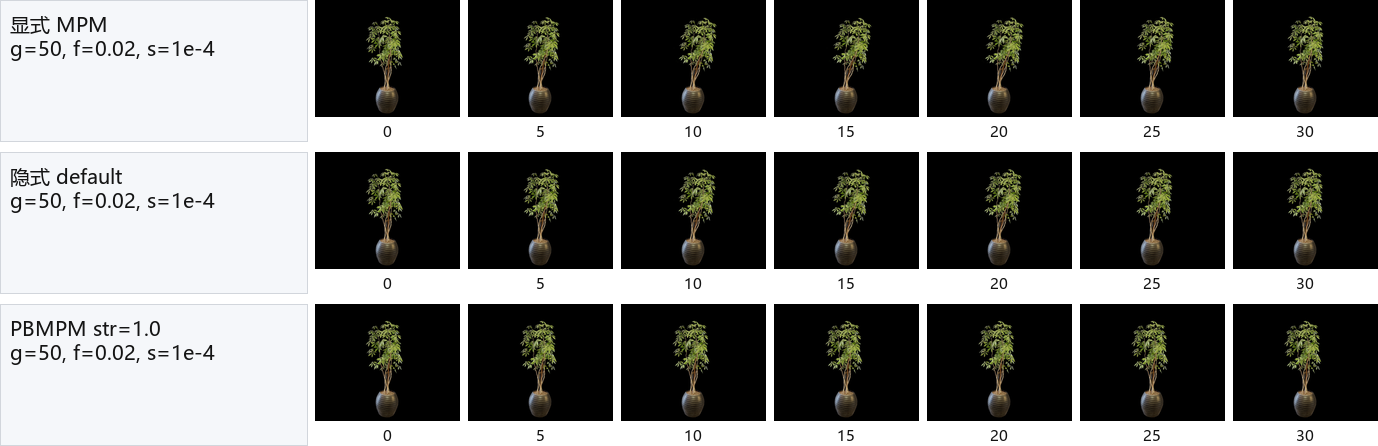
\includegraphics[width=\textwidth]{figures/render_strips/group_baseline.png}
    \caption{baseline 下三类方法的渲染关键帧对比。每行从左到右为第 $0,5,10,15,20,25,30$ 帧。}
    \label{fig:baseline-render-strips}
\end{figure}
\FloatBarrier

% BEGIN RENDER_VISUAL_NOTES fig:baseline-render-strips
从图~\ref{fig:baseline-render-strips} 可以看到，显式 MPM 与隐式 MPM 的树体弯曲更明显，而 PBMPM 在 baseline 下的形变幅度明显偏小。这说明三类方法的 success 不能直接等同于视觉运动强度一致，比较耗时时需要同时检查形变幅度。
% END RENDER_VISUAL_NOTES





三类方法在共享基准点上均能完成仿真，且未出现 NaN 或 Inf。较突出的问题是隐式法耗时显著增加，由于 i-PhysGaussian 未开源，本文实现的预条件、线搜索和失败保护策略仍依赖经验调参，后续调参结果将在其他实验中进一步讨论。PBMPM 的运动幅度明显小于显式法和隐式法，这与其投影式更新机制以及当前采用的 \texttt{strength} 参数设置有关，后续也会讨论。


\subsection{$n_{\mathrm{grid}}$ 消融}

固定
\[
    \Delta t_{\mathrm{frame}}=0.02,\qquad
    \Delta t_{\mathrm{sub}}=10^{-4},
\]
改变网格分辨率 $n_{\mathrm{grid}}$，得到表~\ref{tab:grid-ablation}。

\begin{table}[H]
\centering
\caption{$n_{\mathrm{grid}}$ 消融结果}
\label{tab:grid-ablation}
\small
\begin{tabular}{lccccccc}
\toprule
方法 & $n_{\mathrm{grid}}$ & 成功 & 总耗时/s & 实际/理论子步 & 最大位移 & 最大速度 & $r_{\mathrm{bbox}}$ \\
\midrule
显式 MPM & $25$ & 是 & $63.26$ & $6000/6000$ & $0.1098$ & $0.9818$ & $1.0006$ \\
显式 MPM & $50$ & 是 & $62.95$ & $6000/6000$ & $0.3787$ & $2.1449$ & $1.0318$ \\
显式 MPM & $100$ & 否 & $6.35$ & $1/6000$ & $0.0000$ & -- & $1.0000$ \\
\midrule
隐式 MPM & $25$ & 是 & $902.45$ & $6072/6000$ & $0.0998$ & $0.9528$ & $1.0008$ \\
隐式 MPM & $50$ & 是 & $612.54$ & $6014/6000$ & $0.3262$ & $2.0470$ & $1.0247$ \\
隐式 MPM & $100$ & 否 & $2716.00$ & --$/6000$ & -- & -- & -- \\
\midrule
PBMPM & $25$ & 是 & $39.21$ & $6000/6000$ & $0.0062$ & $0.3094$ & $1.0004$ \\
PBMPM & $50$ & 是 & $46.62$ & $6000/6000$ & $0.0420$ & $1.2264$ & $1.0021$ \\
PBMPM & $100$ & 是 & $74.85$ & $6000/6000$ & $0.1816$ & $3.7080$ & $1.0299$ \\
\bottomrule
\end{tabular}
\end{table}

\begin{figure}[H]
    \centering
    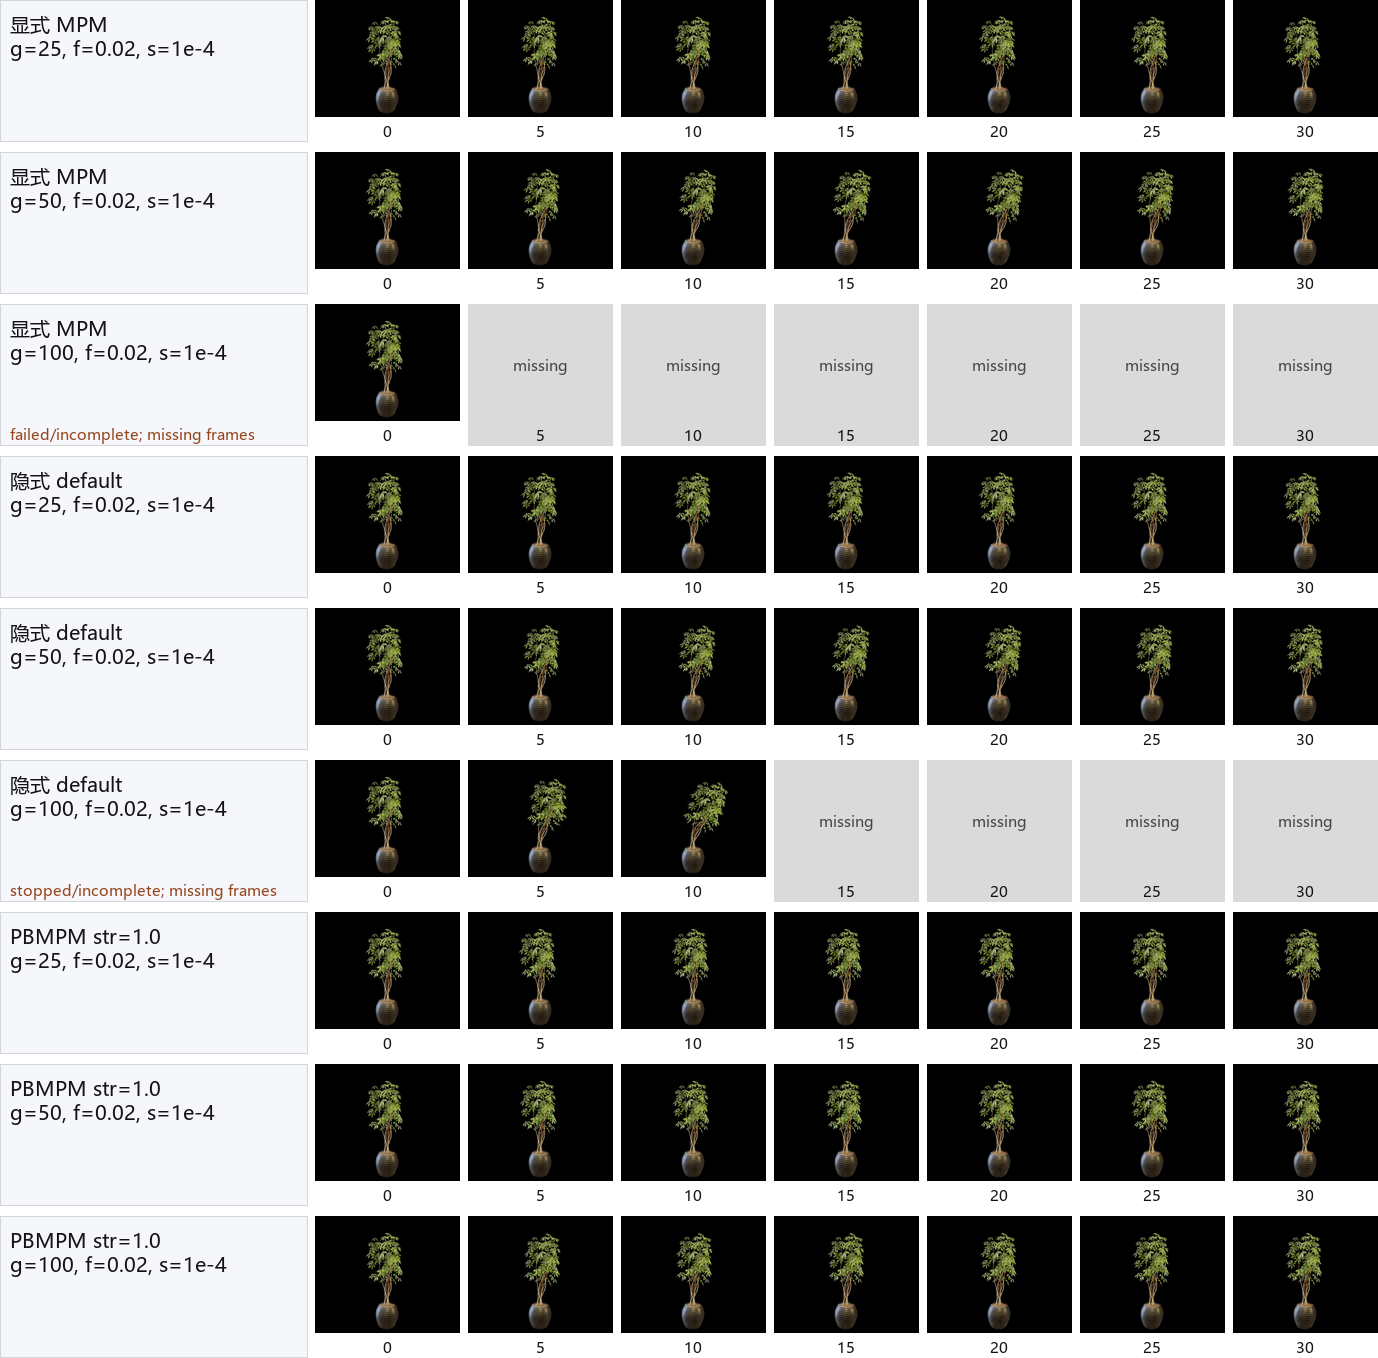
\includegraphics[width=\textwidth,height=0.58\textheight,keepaspectratio]{figures/render_strips/group_grid.png}
    \caption{网格分辨率消融实验的渲染关键帧对比。缺失或中止的帧在图中以灰色占位标注。}
    \label{fig:grid-render-strips}
\end{figure}
\FloatBarrier

% BEGIN RENDER_VISUAL_NOTES fig:grid-render-strips
从图~\ref{fig:grid-render-strips} 看，$n_{\mathrm{grid}}=100$ 时 PBMPM 的枝叶弯曲和整体位移明显增强；显式 MPM 在该设置下只保留首帧，隐式 MPM 也未完整渲染。该组结果提示细网格会同时提高代价和 motion 风险。
% END RENDER_VISUAL_NOTES





网格分辨率对三类方法的影响不同。显式 MPM 在 $n_{\mathrm{grid}}=100$ 时立即触发 \texttt{explicit\_cfl\_limit\_exceeded}，这是因为网格变细后网格尺度 $h$ 变小，CFL 条件中的 $\Delta t/h$ 增大，使显式法稳定条件更严格。隐式 MPM 在 $n_{\mathrm{grid}}=100$ 时运行过慢而被中止，根据历史输出，它的求解是成功的。PBMPM 三组均成功，但随着网格变细，内层迭代数、耗时和运动幅度均增加，说明网格尺度不仅影响空间分辨率，也会影响投影传播和参数映射后的运动幅度。

从运动幅度看，三类方法在 $n_{\mathrm{grid}}=25$ 时位移都偏小，说明粗网格会带来更强的数值平滑或运动抑制；$n_{\mathrm{grid}}=50$ 是本实验中较平衡的选择。$n_{\mathrm{grid}}=100$ 对显式法和隐式法都带来明显代价，而 PBMPM 虽然成功，但速度和加速度明显上升，后续仍需结合视觉结果判断其 motion 质量。

\subsection{$\Delta t_{\mathrm{frame}}$ 消融}

固定
\[
    n_{\mathrm{grid}}=50,\qquad
    \Delta t_{\mathrm{sub}}=10^{-4},
\]
改变帧时间步长 $\Delta t_{\mathrm{frame}}$，结果见表~\ref{tab:frame-dt-ablation}。

\begin{table}[H]
\centering
\caption{$\Delta t_{\mathrm{frame}}$ 消融结果}
\label{tab:frame-dt-ablation}
\small
\begin{tabular}{lccccccc}
\toprule
方法 & $\Delta t_{\mathrm{frame}}$ & 成功 & 总耗时/s & 实际/理论子步 & 最大位移 & 最大速度 & 最大加速度 \\
\midrule
显式 MPM & $0.02$ & 是 & $62.95$ & $6000/6000$ & $0.3787$ & $2.1449$ & $35.28$ \\
显式 MPM & $0.04$ & 是 & $115.61$ & $12000/12000$ & $0.3777$ & $2.1198$ & $17.52$ \\
显式 MPM & $0.06$ & 是 & $163.34$ & $18000/18000$ & $0.3771$ & $1.8392$ & $7.86$ \\
\midrule
隐式 MPM & $0.02$ & 是 & $612.54$ & $6014/6000$ & $0.3262$ & $2.0470$ & $35.48$ \\
隐式 MPM & $0.04$ & 是 & $1391.95$ & $12032/12000$ & $0.3262$ & $2.0044$ & $18.32$ \\
隐式 MPM & $0.06$ & 是 & $2130.76$ & $18040/18000$ & $0.3251$ & $1.7846$ & $7.97$ \\
\midrule
PBMPM & $0.02$ & 是 & $46.62$ & $6000/6000$ & $0.0420$ & $1.2264$ & $32.22$ \\
PBMPM & $0.04$ & 是 & $87.74$ & $12000/12000$ & $0.0416$ & $0.9328$ & $21.05$ \\
PBMPM & $0.06$ & 是 & $125.13$ & $18000/18000$ & $0.0420$ & $0.7005$ & $13.51$ \\
\bottomrule
\end{tabular}
\end{table}

\begin{figure}[H]
    \centering
    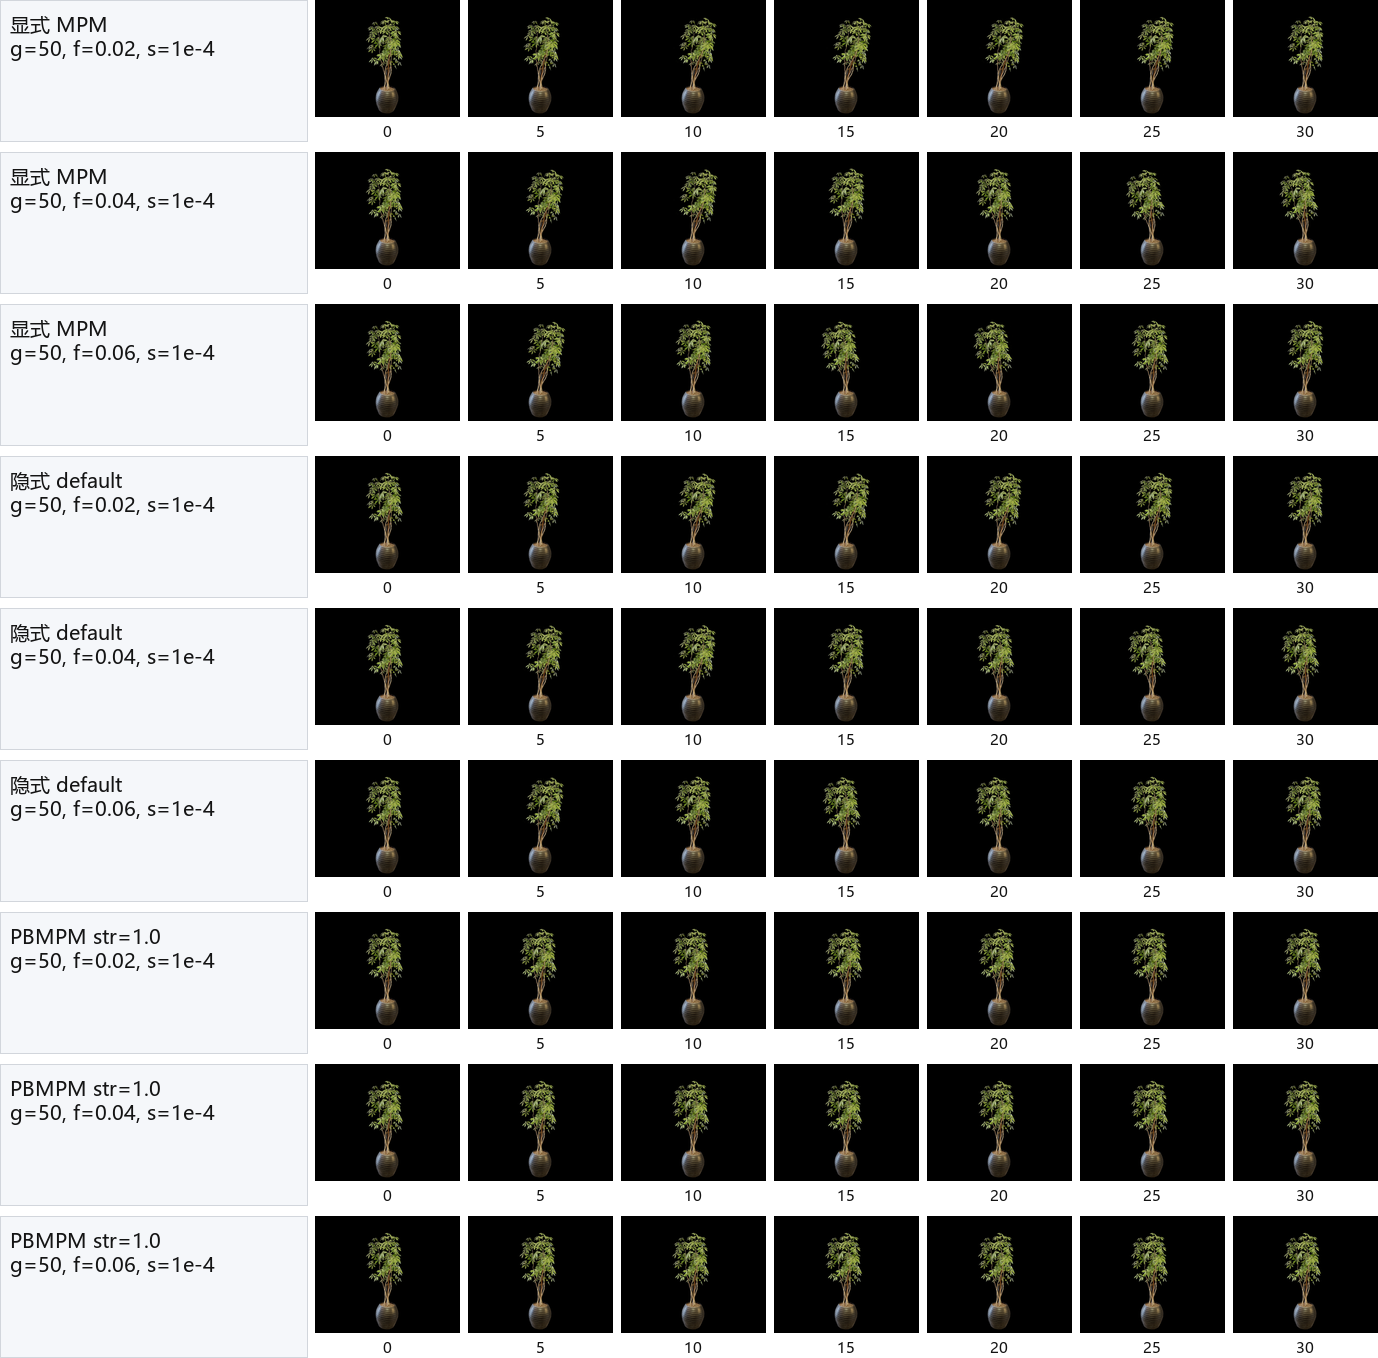
\includegraphics[width=\textwidth,height=0.45\textheight,keepaspectratio]{figures/render_strips/group_frame_dt.png}
    \caption{帧时间步长消融实验的渲染关键帧对比。每行对应一个方法和一个 $\Delta t_{\mathrm{frame}}$ 设置。}
    \label{fig:frame-dt-render-strips}
\end{figure}
\FloatBarrier

% BEGIN RENDER_VISUAL_NOTES fig:frame-dt-render-strips
从图~\ref{fig:frame-dt-render-strips} 看，增大 $\Delta t_{\mathrm{frame}}$ 后主要变化来自总仿真时长增加，三类方法的主要形变趋势没有发生突变。
% END RENDER_VISUAL_NOTES





在本组实验中，$\Delta t_{\mathrm{frame}}$ 增大没有引发三类方法失败，因为子步长 $\Delta t_{\mathrm{sub}}$ 保持为 $10^{-4}$，单子步稳定性没有变差。$\Delta t_{\mathrm{frame}}$ 主要改变每帧包含的子步数和总子步数，因此三类方法总耗时均随 $\Delta t_{\mathrm{frame}}$ 增大而增加。

\subsection{$\Delta t_{\mathrm{sub}}$ 消融}

固定
\[
    n_{\mathrm{grid}}=50,\qquad
    \Delta t_{\mathrm{frame}}=0.02,
\]
改变子步长 $\Delta t_{\mathrm{sub}}$，结果如表~\ref{tab:substep-dt-ablation} 所示。

\begin{table}[H]
\centering
\caption{$\Delta t_{\mathrm{sub}}$ 消融结果}
\label{tab:substep-dt-ablation}
\small
\begin{tabular}{lccccccc}
\toprule
方法 & $\Delta t_{\mathrm{sub}}$ & 成功 & 总耗时/s & 实际/理论子步 & 最大位移 & 最大速度 & 最大加速度 \\
\midrule
显式 MPM & $10^{-4}$ & 是 & $62.95$ & $6000/6000$ & $0.3787$ & $2.1449$ & $35.28$ \\
显式 MPM & $5\times10^{-4}$ & 否 & $6.22$ & $1/1200$ & $0.0000$ & -- & -- \\
显式 MPM & $10^{-3}$ & 否 & $6.42$ & $1/600$ & $0.0000$ & -- & -- \\
\midrule
隐式 MPM & $10^{-4}$ & 是 & $612.54$ & $6014/6000$ & $0.3262$ & $2.0470$ & $35.48$ \\
隐式 MPM & $5\times10^{-4}$ & 是 & $1261.55$ & $1256/1200$ & $1.8532$ & $11.4053$ & $207.84$ \\
隐式 MPM & $10^{-3}$ & 否 & $533.69$ & $248/600$ & $1.3781$ & $21.1207$ & $592.98$ \\
\midrule
PBMPM & $10^{-4}$ & 是 & $46.62$ & $6000/6000$ & $0.0420$ & $1.2264$ & $32.22$ \\
PBMPM & $5\times10^{-4}$ & 是 & $38.01$ & $1200/1200$ & $0.4802$ & $7.5338$ & $136.23$ \\
PBMPM & $10^{-3}$ & 是 & $21.56$ & $600/600$ & $1.6811$ & $16.2235$ & $281.62$ \\
\bottomrule
\end{tabular}
\end{table}

\begin{figure}[H]
    \centering
    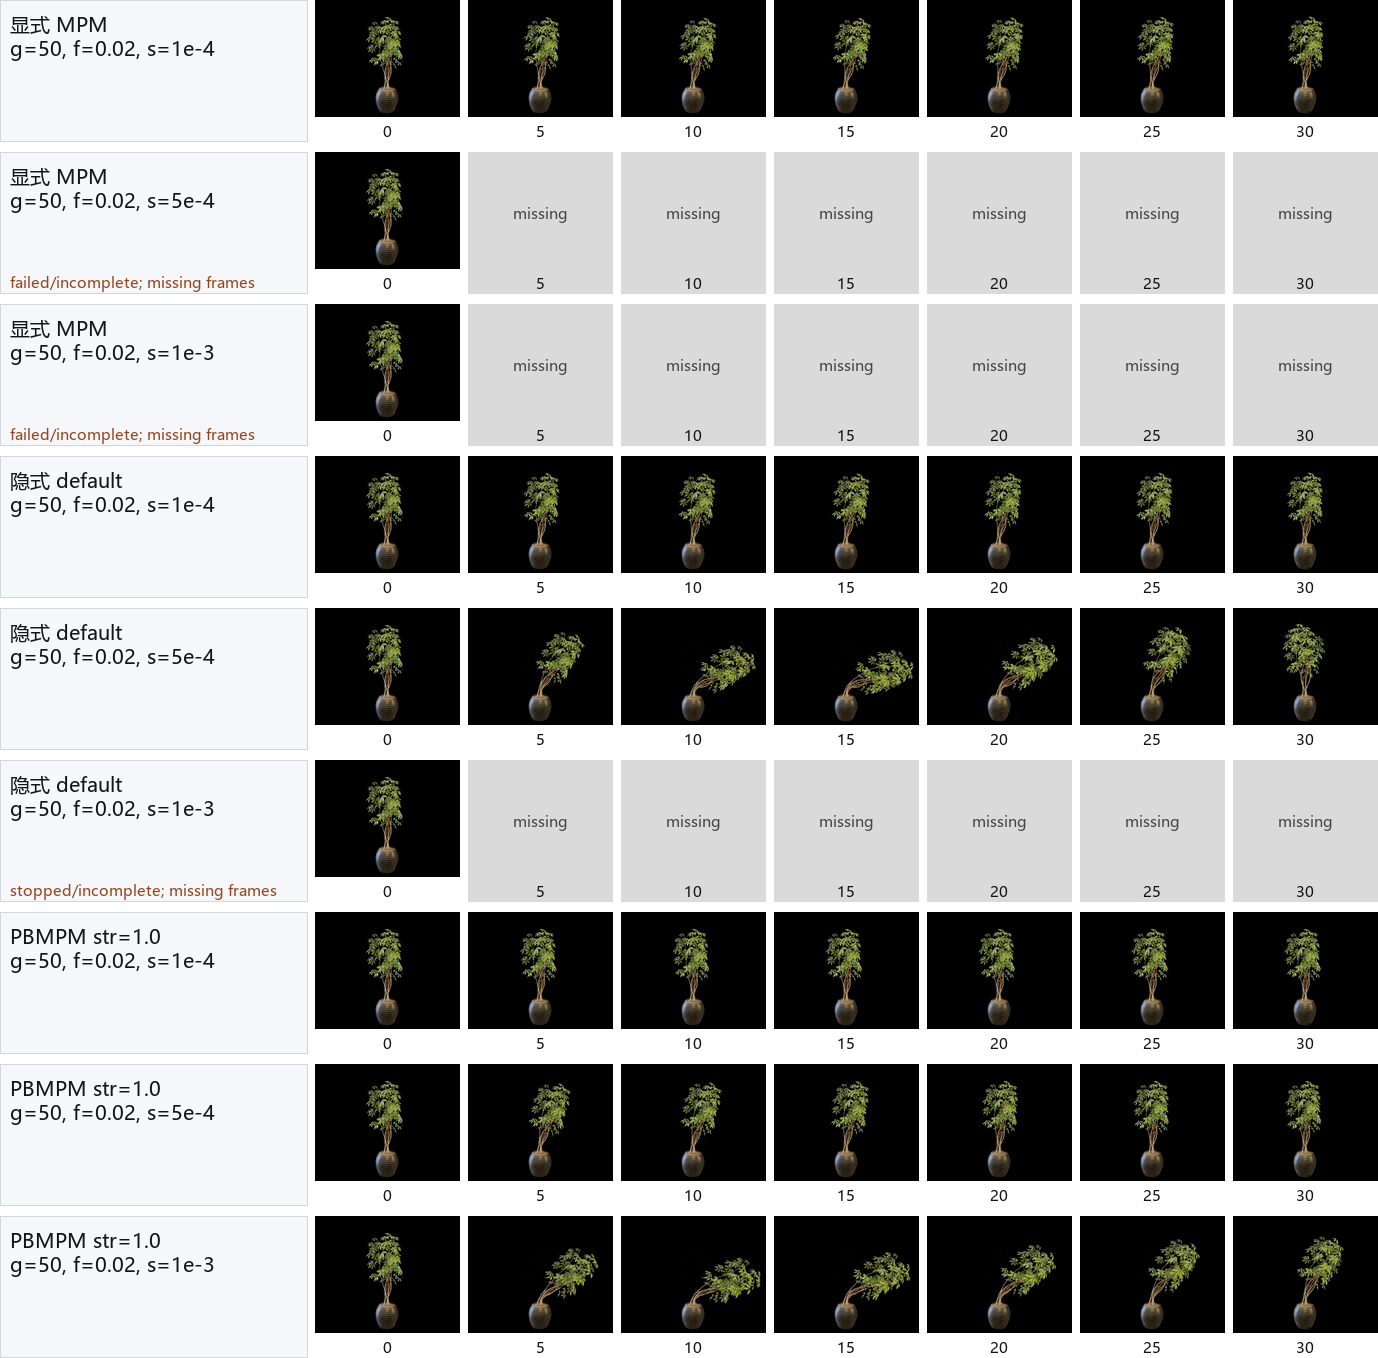
\includegraphics[width=\textwidth,height=0.45\textheight,keepaspectratio]{figures/render_strips/group_substep_dt.png}
    \caption{子步长消融实验的渲染关键帧对比。失败或未完整生成的 run 按已有帧展示，并在缺失位置显式标注。}
    \label{fig:substep-dt-render-strips}
\end{figure}
\FloatBarrier

% BEGIN RENDER_VISUAL_NOTES fig:substep-dt-render-strips
从图~\ref{fig:substep-dt-render-strips} 看，大子步对视觉质量影响更直接。显式 MPM 在大子步下立即失败；隐式 MPM 和 PBMPM 虽能产生 motion，但树体弯曲明显放大，尤其 $\Delta t_{\mathrm{sub}}=10^{-3}$ 时已经出现过度弯曲。
% END RENDER_VISUAL_NOTES





显式 MPM 在 $\Delta t_{\mathrm{sub}}=5\times10^{-4}$ 和 $10^{-3}$ 时均在第一个子步触发 CFL 限制，对单子步长度非常敏感。

隐式 MPM 在 $\Delta t_{\mathrm{sub}}=5\times10^{-4}$ 下仍能完成仿真，对应相对于基准子步长 $10^{-4}$ 的 $5\times$ 时间步放大，但该 run 的 motion 质量已经明显下降。同时，实际子步数为 $1256/1200$，并出现 $93$ 次 fallback、$3834$ 次 GMRES 内层未收敛和 $1$ 次 line search failure，说明该设置虽然成功提交 motion，但求解过程已接近不稳定区域。

当 $\Delta t_{\mathrm{sub}}=10^{-3}$ 时，时间步放大倍数达到 $10\times$，隐式法只完成 $248/600$ 个子步，最终因 \texttt{newton\_not\_converged} 失败。该失败与过大的时间步导致非线性残差更难求解有关，也与当前实现中的 GMRES 容差、最大迭代数、线搜索策略和收敛阈值设置有关。由于 i-PhysGaussian 原文未开源，本文实现中的预条件器、fallback 和收敛判定仍依赖经验调参；本组默认参数相对保守，因此在 $10\times$ 时间步下未能稳定完成仿真。总体来看，当前隐式实现已经验证了相对显式法更大的稳定区域，但尚未达到原文报告的最高 $20\times$ 时间步尺度。

PBMPM 在三种 $\Delta t_{\mathrm{sub}}$ 设置下均能完成仿真，并且随着子步长增大，总子步数减少，总耗时下降。但PBMPM缺少失败条件，实际成功标准依赖视觉效果。

\subsection{小结}
$n_{\mathrm{grid}}$ 主要影响空间离散尺度和计算自由度：对显式 MPM，网格加密会减小 $h$，从而提高 CFL 失稳风险；对隐式 MPM，网格加密会增加残差计算和 GMRES 求解代价；对 PBMPM，网格加密会改变投影传播效果，并使运动幅度和耗时上升。

$\Delta t_{\mathrm{frame}}$ 主要影响总仿真时长和总子步数。在固定 $\Delta t_{\mathrm{sub}}$ 时，它不会直接改变单子步稳定性，因此三类方法均能完成对应实验，但总耗时随 $\Delta t_{\mathrm{frame}}$ 增大而增加。

$\Delta t_{\mathrm{sub}}$ 是最直接影响稳定性和运动质量的参数。对显式 MPM，子步长增大会直接提高 CFL 数并导致失败；对隐式 MPM，适度增大子步长可以体现更大的稳定区域，但过大时会造成 Newton--GMRES 收敛困难和运动放大；对 PBMPM，子步长增大虽然减少总子步数并降低耗时，但会显著放大位移、速度和加速度。

\section{隐式 MPM 容差参数调参分析}

在baseline
\[
    n_{\mathrm{grid}}=50,\qquad
    \Delta t_{\mathrm{frame}}=0.02,\qquad
    \Delta t_{\mathrm{sub}}=10^{-4}
\]
下，本文比较了 \texttt{relaxed}、\texttt{default} 和 \texttt{strict} 三种隐式容差设置。三组实验均能完成仿真，且最终 motion 指标几乎一致，但求解代价差异明显。

\begin{table}[H]
\centering
\caption{隐式 MPM 容差设置对求解代价的影响}
\label{tab:implicit-profile-cost}
\small
\begin{tabular}{lccccccc}
\toprule
Profile & 总耗时/s & 实际/理论子步 & Newton & GMRES & GMRES 未收敛 & fallback & line search failure \\
\midrule
\texttt{relaxed} & $400.21$ & $6008/6000$ & $6773$ & $27474$ & $769$ & $15$ & $1$ \\
\texttt{default} & $612.54$ & $6014/6000$ & $7931$ & $42523$ & $1203$ & $15$ & $0$ \\
\texttt{strict} & $2614.06$ & $6020/6000$ & $21941$ & $157741$ & $2415$ & $19$ & $1$ \\
\bottomrule
\end{tabular}
\end{table}


从 trace 可以看到，\texttt{relaxed} 的主要作用是提前接受已经足够好的隐式子步，从而减少不必要的 Newton--GMRES 迭代。它的 Newton 总迭代数为 $6773$，低于 \texttt{default} 的 $7931$；GMRES 总迭代数为 $27474$，相比 \texttt{default} 减少约 $35\%$；总耗时也从 $612.54\,\mathrm{s}$ 降到 $400.21\,\mathrm{s}$。同时，\texttt{relaxed} 的自适应子步尝试较少，实际子步数为 $6008/6000$，对应 $4$ 次未收敛尝试被拆分处理；而 \texttt{default} 为 $6014/6000$，对应 $7$ 次未收敛尝试。

\begin{table}[H]
\centering
\caption{隐式 MPM 容差设置对残差和 motion 的影响}
\label{tab:implicit-profile-motion}
\small
\begin{tabular}{lcccccc}
\toprule
Profile & 相对残差均值 & RMS 残差均值 & 最大位移 & 平均位移 & 最大速度 & 最大加速度 \\
\midrule
\texttt{relaxed} & $0.139$ & $8.53\times10^{-5}$ & $0.3262$ & $0.0666$ & $2.0468$ & $35.48$ \\
\texttt{default} & $0.128$ & $7.68\times10^{-5}$ & $0.3262$ & $0.0666$ & $2.0470$ & $35.48$ \\
\texttt{strict} & $0.073$ & $4.33\times10^{-5}$ & $0.3263$ & $0.0666$ & $2.0471$ & $35.48$ \\
\bottomrule
\end{tabular}
\end{table}

\begin{figure}[H]
    \centering
    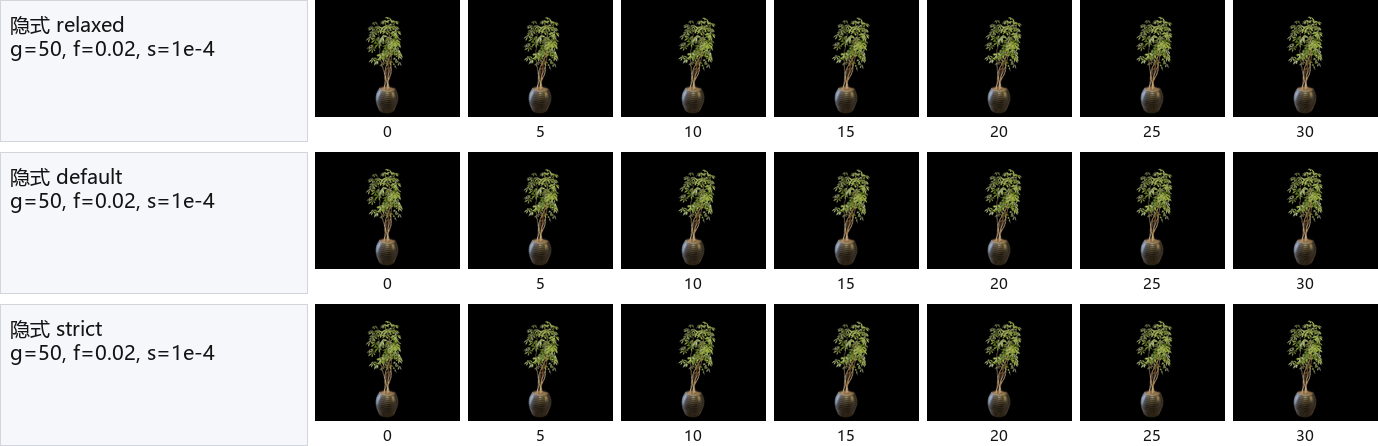
\includegraphics[width=\textwidth]{figures/render_strips/group_implicit_tolerance.png}
    \caption{隐式 MPM tolerance profile 调参的渲染关键帧对比。}
    \label{fig:implicit-tolerance-render-strips}
\end{figure}
\FloatBarrier

% BEGIN RENDER_VISUAL_NOTES fig:implicit-tolerance-render-strips
从图~\ref{fig:implicit-tolerance-render-strips} 看，三组 tolerance profile 的渲染差异很小，与 motion 指标接近一致；更严格的残差设置主要提高数值精度，并未带来明显视觉改善。
% END RENDER_VISUAL_NOTES





残差方面，\texttt{relaxed} 的相对残差均值和 RMS 残差均值略高于 \texttt{default}，说明它确实降低了隐式方程的求解精度要求。但从最大位移、平均位移、最大速度和最大加速度看，三组 profile 的 motion 指标几乎没有差异。因此，在当前花盆场景和该基准点下，\texttt{strict} 主要提升残差精度，却没有带来可观察的运动质量改善；\texttt{relaxed} 则以较小的残差精度损失显著降低了计算代价。





% BEGIN PBMPM_EVAL_SECTION
\section{PBMPM 参数调参分析}
此处的超松弛系数与dt解耦了。
由于离线渲染包中的相机移动未关闭，因此本节插图会有轻微视角旋转，但是不影响实际数据。

\subsection{relaxation=1.5 下的通用表现}

首先固定 $s_{\mathrm{str}}=1.0$、$\omega=1.5$。网格消融结果见表~\ref{tab:pbmpm-common-grid-rel15}。
\begin{table}[H]
\centering
\caption{PBMPM 在 $\omega=1.5$ 下的网格消融}
\label{tab:pbmpm-common-grid-rel15}
\small
\resizebox{\textwidth}{!}{%
\begin{tabular}{lccccccccc}
\toprule
$n_{\mathrm{grid}}$ & 成功 & 内步/理论 & 投影迭代 & 耗时/s & $d_{\max}$ & $\bar d$ & $v_{\max}$ & $a_{\max}$ & $r_{\mathrm{bbox}}$ \\
\midrule
$25$ & 是 & 6000/6000 & 3.0 & 40.65 & 0.0051 & 0.0008 & 0.257 & 15.72 & 1.0005 \\
$50$ & 是 & 6000/6000 & 5.0 & 46.88 & 0.0356 & 0.0023 & 1.208 & 37.17 & 1.0016 \\
$100$ & 是 & 6000/6000 & 11.00 & 75.91 & 0.1625 & 0.0154 & 3.680 & 76.12 & 1.0218 \\
\bottomrule
\end{tabular}%
}
\end{table}
\begin{figure}[H]
    \centering
    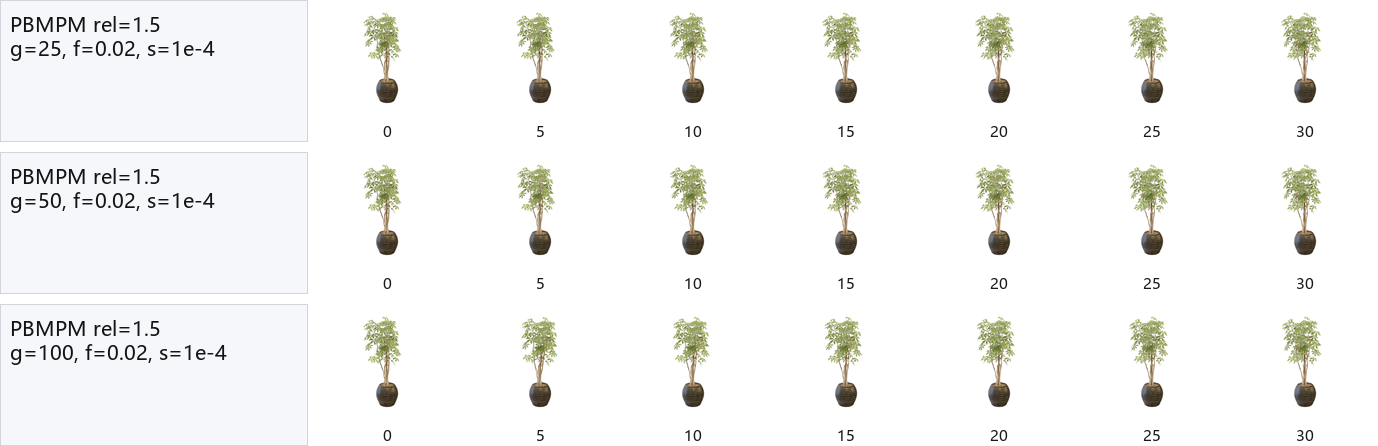
\includegraphics[width=\textwidth,height=0.31\textheight,keepaspectratio]{figures/render_strips/group_pbmpm_eval_common_grid.png}
    \caption{PBMPM 在 $\omega=1.5$ 下的网格消融渲染关键帧。每行从左到右为第 $0,5,10,15,20,25,30$ 帧。}
    \label{fig:pbmpm-eval-common-grid}
\end{figure}
\FloatBarrier
可以看到，$n_{\mathrm{grid}}=100$ 时投影迭代次数增至 $11$，最大位移、速度和加速度均明显高于 $25$ 与 $50$。这说明 relaxation 解耦后，细网格下 PBMPM 仍会放大 motion；视觉上树体弯曲也更明显。

子步长消融结果见表~\ref{tab:pbmpm-common-substep-rel15}。
\begin{table}[H]
\centering
\caption{PBMPM 在 $\omega=1.5$ 下的子步长消融}
\label{tab:pbmpm-common-substep-rel15}
\small
\resizebox{\textwidth}{!}{%
\begin{tabular}{lccccccccc}
\toprule
$\Delta t_{\mathrm{sub}}$ & 成功 & 内步/理论 & 投影迭代 & 耗时/s & $d_{\max}$ & $\bar d$ & $v_{\max}$ & $a_{\max}$ & $r_{\mathrm{bbox}}$ \\
\midrule
$10^{-4}$ & 是 & 6000/6000 & 5.0 & 46.88 & 0.0356 & 0.0023 & 1.208 & 37.17 & 1.0016 \\
$5\times10^{-4}$ & 是 & 1200/1200 & 24.00 & 38.66 & 0.4417 & 0.0070 & 7.568 & 133.9 & 1.0071 \\
$10^{-3}$ & 是 & 600/600 & 24.00 & 22.42 & 1.6493 & 0.2556 & 16.11 & 313.2 & 1.2151 \\
\bottomrule
\end{tabular}%
}
\end{table}
\begin{figure}[H]
    \centering
    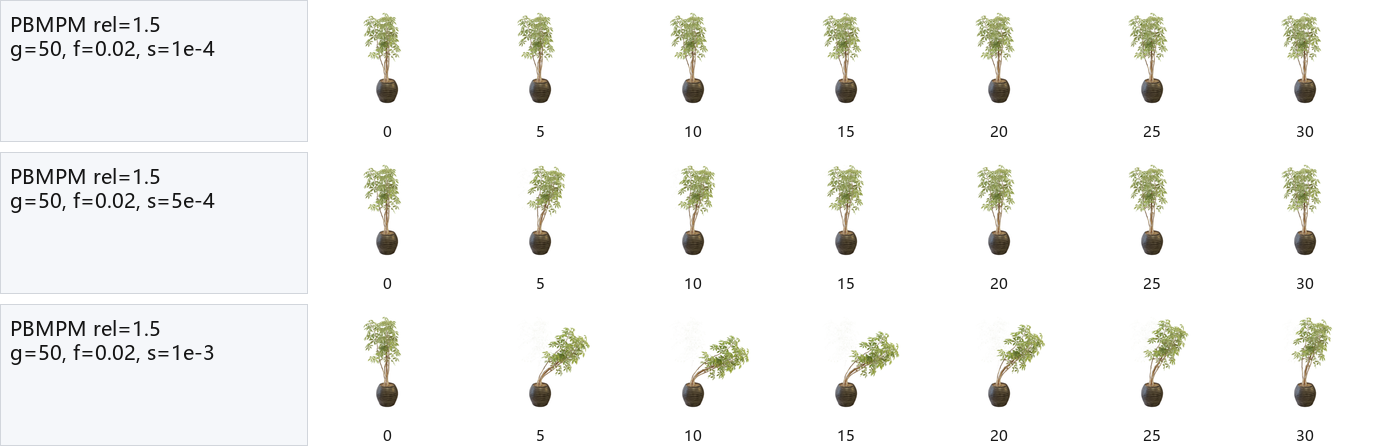
\includegraphics[width=\textwidth,height=0.31\textheight,keepaspectratio]{figures/render_strips/group_pbmpm_eval_common_substep.png}
    \caption{PBMPM 在 $\omega=1.5$ 下的子步长消融渲染关键帧。}
    \label{fig:pbmpm-eval-common-substep}
\end{figure}
\FloatBarrier
$\Delta t_{\mathrm{sub}}=10^{-3}$ 虽然成功完成，但最大位移达到 $1.6493$，bbox 体积比达到 $1.2151$，图中树体已经出现明显过度弯曲。因此 PBMPM 的 success 只说明程序生成了 motion，不等价于 motion 合理。

\subsection{relaxation 参数实验}

在 $n_{\mathrm{grid}}=100$ 下扫描 $\omega$，结果见表~\ref{tab:pbmpm-relax-grid100}。
\begin{table}[H]
\centering
\caption{PBMPM 在 $n_{\mathrm{grid}}=100$ 下的 relaxation 实验}
\label{tab:pbmpm-relax-grid100}
\small
\resizebox{\textwidth}{!}{%
\begin{tabular}{lccccccccc}
\toprule
$\omega$ & 成功 & 内步/理论 & 投影迭代 & 耗时/s & $d_{\max}$ & $\bar d$ & $v_{\max}$ & $a_{\max}$ & $r_{\mathrm{bbox}}$ \\
\midrule
$0.0$ & 是 & 6000/6000 & 11.00 & 77.44 & 0.3387 & 0.1998 & 4.173 & 66.54 & 1.0647 \\
$1.0$ & 是 & 6000/6000 & 11.00 & 75.50 & 0.1725 & 0.0255 & 3.695 & 70.87 & 1.0267 \\
$1.5$ & 是 & 6000/6000 & 11.00 & 75.91 & 0.1625 & 0.0154 & 3.680 & 76.12 & 1.0218 \\
$2.0$ & 是 & 6000/6000 & 11.00 & 75.93 & 0.1546 & 0.0107 & 3.669 & 79.87 & 1.0187 \\
\bottomrule
\end{tabular}%
}
\end{table}
\begin{figure}[H]
    \centering
    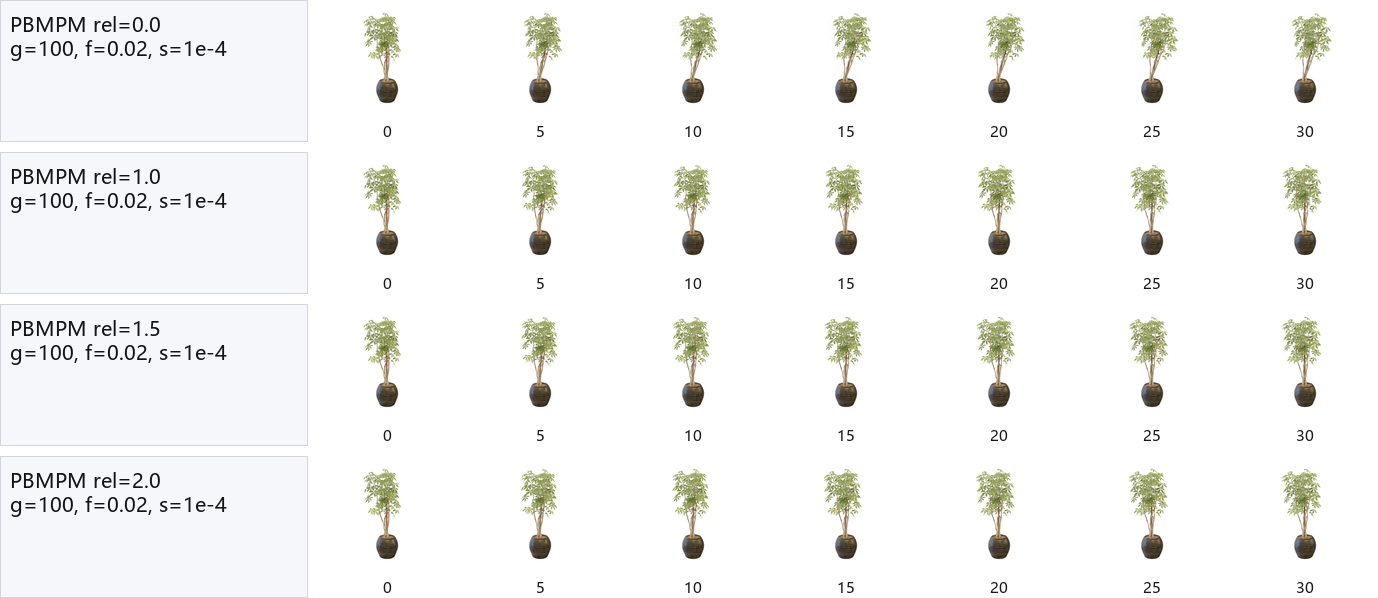
\includegraphics[width=\textwidth,height=0.40\textheight,keepaspectratio]{figures/render_strips/group_pbmpm_eval_relax_grid100.png}
    \caption{PBMPM 在 $n_{\mathrm{grid}}=100$ 下扫描 relaxation 的渲染关键帧。}
    \label{fig:pbmpm-eval-relax-grid100}
\end{figure}
\FloatBarrier
随着 $\omega$ 从 $0$ 增大到 $2$，平均位移从 $0.1998$ 降至 $0.0107$，bbox 体积比从 $1.0647$ 降至 $1.0187$；但最大加速度从 $66.54$ 升至 $79.87$。这说明 relaxation 是关键稳定参数，但较强投影也可能带来更尖锐的局部速度变化。

在 $\Delta t_{\mathrm{sub}}=10^{-3}$ 下扫描 $\omega$，结果见表~\ref{tab:pbmpm-relax-dt001}。
\begin{table}[H]
\centering
\caption{PBMPM 在 $\Delta t_{\mathrm{sub}}=10^{-3}$ 下的 relaxation 实验}
\label{tab:pbmpm-relax-dt001}
\small
\resizebox{\textwidth}{!}{%
\begin{tabular}{lccccccccc}
\toprule
$\omega$ & 成功 & 内步/理论 & 投影迭代 & 耗时/s & $d_{\max}$ & $\bar d$ & $v_{\max}$ & $a_{\max}$ & $r_{\mathrm{bbox}}$ \\
\midrule
$0.0$ & 否 & 137/600 & 24.00 & 10.57 & 1.6918 & 1.0298 & 17.98 & 151.0 & 2.4005 \\
$1.0$ & 是 & 600/600 & 24.00 & 22.78 & 1.6811 & 0.3767 & 16.22 & 281.6 & 1.3003 \\
$1.5$ & 是 & 600/600 & 24.00 & 22.42 & 1.6493 & 0.2556 & 16.11 & 313.2 & 1.2151 \\
$2.0$ & 是 & 600/600 & 24.00 & 22.80 & 1.5650 & 0.1281 & 16.03 & 329.7 & 1.0991 \\
\bottomrule
\end{tabular}%
}
\end{table}
\begin{figure}[H]
    \centering
    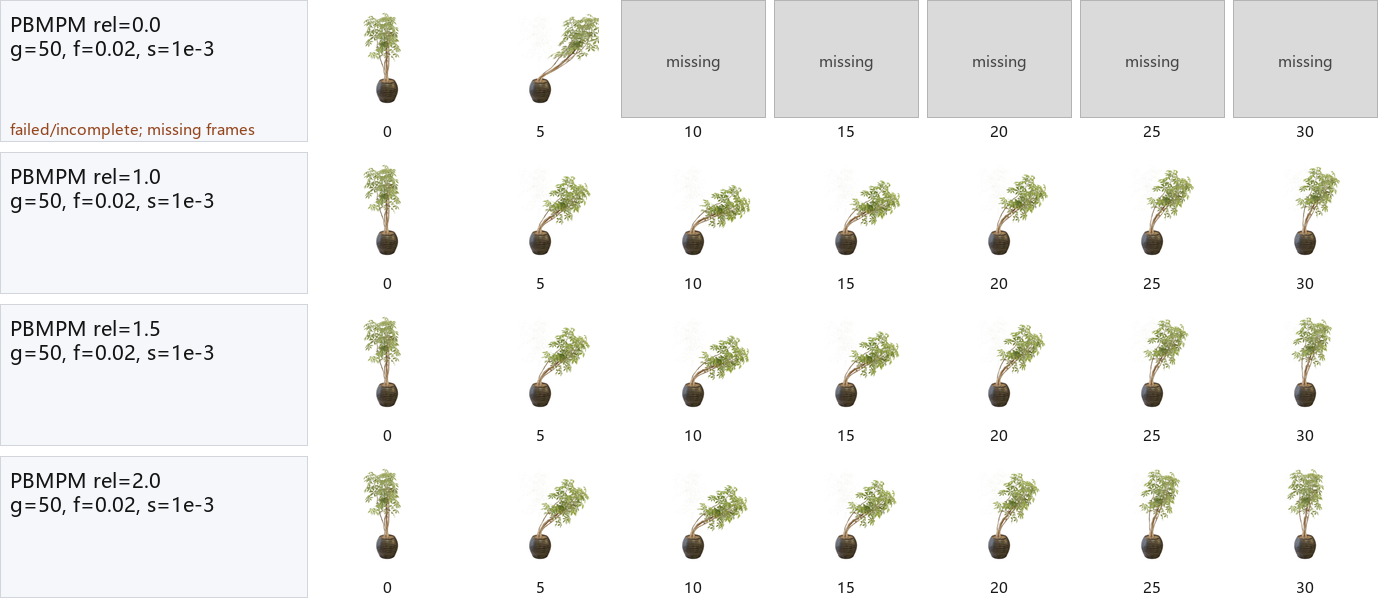
\includegraphics[width=\textwidth,height=0.40\textheight,keepaspectratio]{figures/render_strips/group_pbmpm_eval_relax_dt001.png}
    \caption{PBMPM 在 $\Delta t_{\mathrm{sub}}=10^{-3}$ 下扫描 relaxation 的渲染关键帧；缺失帧以灰色占位表示。}
    \label{fig:pbmpm-eval-relax-dt001}
\end{figure}
\FloatBarrier
$\omega=0$ 的 run 只生成 $7$ 帧并以 \texttt{exit\_code\_-6} 失败，$\omega=1,1.5,2$ 均能完成。增大 $\omega$ 可显著降低平均位移和 bbox 膨胀，但最大位移仍保持在 $1.5$ 以上，说明 relaxation 解耦改善了大时间步稳定性，却不能完全消除大时间步导致的 motion 放大。

\subsection{strength 参数实验}

在 $n_{\mathrm{grid}}=100$ 下扫描 strength，结果见表~\ref{tab:pbmpm-strength-grid100}。
\begin{table}[H]
\centering
\caption{PBMPM 在 $n_{\mathrm{grid}}=100$ 下的 strength 实验}
\label{tab:pbmpm-strength-grid100}
\small
\resizebox{\textwidth}{!}{%
\begin{tabular}{lccccccccc}
\toprule
$s_{\mathrm{str}}$ & 成功 & 内步/理论 & 投影迭代 & 耗时/s & $d_{\max}$ & $\bar d$ & $v_{\max}$ & $a_{\max}$ & $r_{\mathrm{bbox}}$ \\
\midrule
$0.25$ & 是 & 6000/6000 & 5.0 & 44.26 & 0.2650 & 0.0525 & 3.990 & 57.77 & 1.0419 \\
$0.50$ & 是 & 6000/6000 & 8.0 & 60.08 & 0.2008 & 0.0282 & 3.825 & 67.15 & 1.0307 \\
$1.00$ & 是 & 6000/6000 & 11.00 & 75.91 & 0.1625 & 0.0154 & 3.680 & 76.12 & 1.0218 \\
$2.00$ & 是 & 6000/6000 & 17.00 & 109.6 & 0.1213 & 0.0072 & 3.431 & 87.57 & 1.0133 \\
$4.00$ & 是 & 6000/6000 & 22.00 & 135.0 & 0.1000 & 0.0041 & 3.242 & 96.73 & 1.0086 \\
\bottomrule
\end{tabular}%
}
\end{table}
\begin{figure}[H]
    \centering
    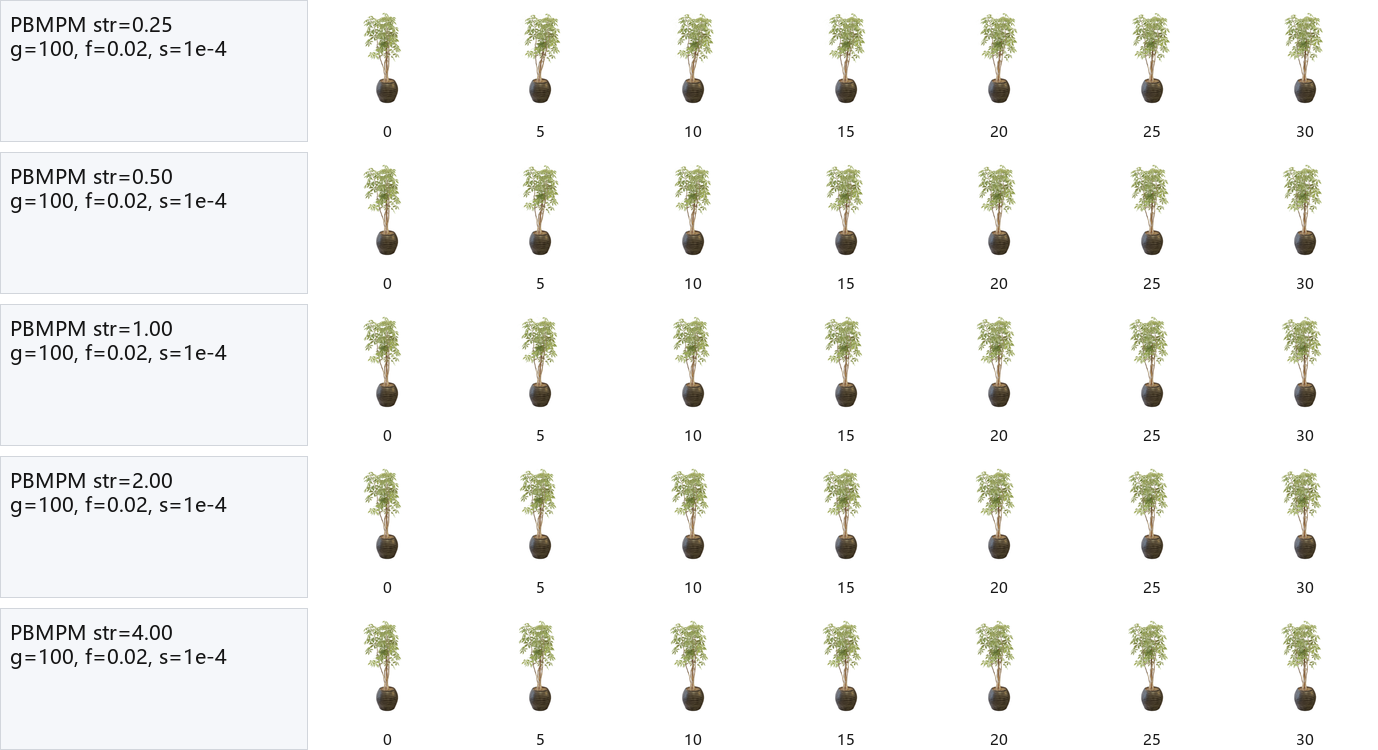
\includegraphics[width=\textwidth,height=0.45\textheight,keepaspectratio]{figures/render_strips/group_pbmpm_eval_strength_grid100.png}
    \caption{PBMPM 在 $n_{\mathrm{grid}}=100$ 下扫描 strength 的渲染关键帧。}
    \label{fig:pbmpm-eval-strength-grid100}
\end{figure}
\FloatBarrier
strength 从 $0.25$ 增大到 $4.0$ 时，投影迭代次数从 $5$ 增至 $22$，平均位移从 $0.0525$ 降至 $0.0041$，bbox 体积比从 $1.0419$ 降至 $1.0086$。因此在细网格设置下，strength 对约束强度和形变幅度有明显作用；同时最大加速度随 strength 增大而升高，说明更强投影会提高局部运动尖峰风险。

在 $\Delta t_{\mathrm{sub}}=10^{-3}$ 下扫描 strength，结果见表~\ref{tab:pbmpm-strength-dt001}。
\begin{table}[H]
\centering
\caption{PBMPM 在 $\Delta t_{\mathrm{sub}}=10^{-3}$ 下的 strength 实验}
\label{tab:pbmpm-strength-dt001}
\small
\resizebox{\textwidth}{!}{%
\begin{tabular}{lccccccccc}
\toprule
$s_{\mathrm{str}}$ & 成功 & 内步/理论 & 投影迭代 & 耗时/s & $d_{\max}$ & $\bar d$ & $v_{\max}$ & $a_{\max}$ & $r_{\mathrm{bbox}}$ \\
\midrule
$0.25$ & 是 & 600/600 & 24.00 & 22.56 & 1.6696 & 0.3001 & 16.15 & 303.4 & 1.2472 \\
$0.50$ & 是 & 600/600 & 24.00 & 22.49 & 1.6545 & 0.2648 & 16.11 & 311.4 & 1.2225 \\
$1.00$ & 是 & 600/600 & 24.00 & 22.42 & 1.6493 & 0.2556 & 16.11 & 313.2 & 1.2151 \\
$2.00$ & 是 & 600/600 & 24.00 & 22.74 & 1.6490 & 0.2551 & 16.10 & 313.3 & 1.2148 \\
$4.00$ & 是 & 600/600 & 25.00 & 23.05 & 1.6290 & 0.2443 & 16.08 & 315.5 & 1.2042 \\
\bottomrule
\end{tabular}%
}
\end{table}
\begin{figure}[H]
    \centering
    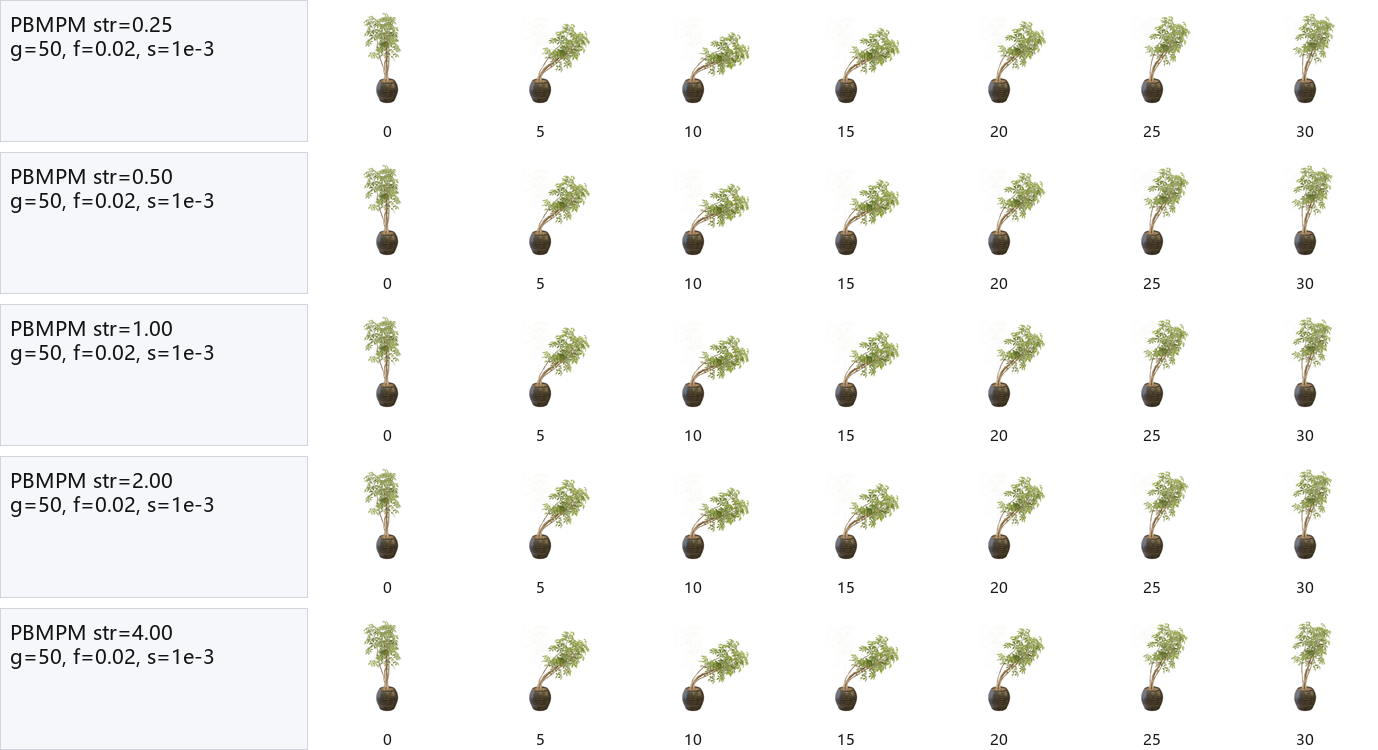
\includegraphics[width=\textwidth,height=0.45\textheight,keepaspectratio]{figures/render_strips/group_pbmpm_eval_strength_dt001.png}
    \caption{PBMPM 在 $\Delta t_{\mathrm{sub}}=10^{-3}$ 下扫描 strength 的渲染关键帧。}
    \label{fig:pbmpm-eval-strength-dt001}
\end{figure}
\FloatBarrier
在大子步设置下，strength 的边际效果有限。strength 从 $0.25$ 增至 $4.0$ 时，平均位移和 bbox 膨胀仅缓慢下降，最大位移仍约为 $1.63$，最大速度约为 $16$。这说明此时自动映射的迭代数已接近上限，主要风险来自过大的 $\Delta t_{\mathrm{sub}}$ 本身，而不是 strength 单独不足。
\begin{table}[H]
\centering
\caption{PBMPM 补充实验中的异常 run}
\label{tab:pbmpm-eval-anomaly}
\small
\resizebox{\textwidth}{!}{%
\begin{tabular}{lccccc}
\toprule
设置 & 成功 & 可用帧 & 内步/理论 & 失败原因 & $r_{\mathrm{bbox}}$ \\
\midrule
$\Delta t_{\mathrm{sub}}=10^{-3},\ \omega=0$ & 否 & 7 & 137/600 & \texttt{exit\_code\_-6} & 2.400 \\
\bottomrule
\end{tabular}%
}
\end{table}
总体而言，PBMPM 的参数评价不能只看 success 或耗时。relaxation 是高风险设置中的关键参数，解耦后可以改善 $n_{\mathrm{grid}}=100$ 和 $\Delta t_{\mathrm{sub}}=10^{-3}$ 的表现；strength 在细网格下有效，在大子步下效果有限。实际使用时仍需同时检查 displacement、velocity、acceleration、bbox 和视觉渲染结果。
% END PBMPM_EVAL_SECTION

\section{感想与感谢}
感觉其实从physgaussian提出引入MPM法后的工作,其实都更倾向于工程上的优化了，最关键的还是从MPM法的视角解决问题。

话虽如此，隐式法引入GRMES避免直接求解病态方程也很妙，这是我第一次见到GRMES这个算法。但是隐式法的各种阈值太多了，太严格了速度会很慢，甚至求解失败，就算能想到方法，调参也是个技术活，而且很费精力。

引入PBMPM其实是之前的弹簧仿真，显式接隐式、隐式接Liu3，自然会想有没有类似的local -global思想，但是因为P2G过程，在这个项目里不能实现类似的预分解，并且也难以定义非常符合物理情况的能量。由于我想引入local-global思想，主要是想保形这一步，尤其是对刚体的保形，能否交给局部求解（类似ARAP），自然会想到能否对object级别的物质点（同时也想到希望在交互里加入object级的属性划分），在G2P过程里，加入刚体约束。而我觉得这种思想应该会有人在传统MPM仿真领域想到，于是搜索得到了PBMPM，虽然和我想的不完全一样（因为它完全没有网格点微分方程求解的步骤），但是个人认为它速度应该很快，在视觉效果上也许能实现比较好的效果，于是选择了遵循原项目的思路，而没有进行大幅度的改变，只是为了参数上的统一，定义了由物理参数到几何参数的转化关系。

哎，比较可惜的是实验其实不是很完善，测试案例也比较单一，没能继续优化PBMPM的实际表现，以及没能调好隐式法的参数，跑的太慢了，等待非常折磨（）。

除了主要的算法之外，其实花在前端的时间也挺多的，虽然仿真可以在服务器上跑，但是3DGS的模型太大了，哪怕只是传变换矩阵，也就是motion，也很大，这一点不知道能不能优化，个人想法可能类似我实现的抓取交互那种proxy编组，当然怎么编也是个问题，现在只是很粗略的邻近搜索，以后也许可以结合法向量找到比较光滑的边界来编组。

其实写这一大段的时候已经很疲倦了，最近事情好多，写的好没激情啊可恶，这个项目我感觉还是很好玩的QAQ，尤其是思考算法的时候。

特别鸣谢codex的会话窗口们不厌其烦的执行我发放的任务（X），尤其是codex能SSH连接服务器，太方便了啊（瘫）
\begin{thebibliography}{9}

\bibitem{kerbl2023gaussian}
Bernhard Kerbl, Georgios Kopanas, Thomas Leimk{\"u}hler, and George Drettakis.
\newblock 3D Gaussian Splatting for Real-Time Radiance Field Rendering.
\newblock \emph{ACM Transactions on Graphics}, 42(4), 2023.

\bibitem{xie2024physgaussian}
Tianyi Xie, Zeshun Zong, Yuxing Qiu, Xuan Li, Yutao Feng, Yin Yang, and Chenfanfu Jiang.
\newblock PhysGaussian: Physics-Integrated 3D Gaussians for Generative Dynamics.
\newblock In \emph{Proceedings of the IEEE/CVF Conference on Computer Vision and Pattern Recognition}, 2024.
\bibitem{cao2026iphysgaussian}
Yicheng Cao, Zhuo Huang, Yu Yao, Yiming Ying, Daoyi Dong, and Tongliang Liu.
\newblock i-PhysGaussian: Implicit Physical Simulation for 3D Gaussian Splatting.
\newblock \emph{arXiv preprint arXiv:2602.17117}, 2026.

\bibitem{lewin2024pbmpm}
Chris Lewin.
\newblock A Position Based Material Point Method.
\newblock In \emph{Special Interest Group on Computer Graphics and Interactive Techniques Conference Talks (SIGGRAPH Talks '24)}, 2024.
\end{thebibliography}

\end{document}
